\documentclass[a4paper,aps,secnumarabic,balancelastpage,amsmath,amssymb,nofootinbib,floatfix]{report}

\usepackage[utf8]{inputenc}
\usepackage{gensymb}
\usepackage{SIunits}
\usepackage{pgfplots}
\pgfplotsset{compat=1.17}
\usepackage{physics}
\usepackage{gensymb}
\usepackage[italian]{babel}
\usepackage{graphicx} 
\usepackage{geometry}
\usepackage{amsfonts}
\usepackage{amsopn}
\usepackage{amsmath}
\usepackage{amssymb}
\usepackage{hyperref}
\usepackage{makeidx}
\usepackage{bm}
\usepackage{fullpage}
\usepackage{subfigure}
\usepackage{graphicx}
\usepackage{subcaption}
\usepackage[export]{adjustbox}
\usepackage{wrapfig}
\usepackage{amsmath}
\usepackage{listings}
\hypersetup{
    colorlinks=true,
    linkcolor=blue,
    filecolor=magenta,      
    urlcolor=cyan,
}
\urlstyle{same}



\makeindex
\selectlanguage{italian}

\begin{document}
\title{\Huge\textbf{Stochastic methods}}
\author{\textbf{Daniele Gelmini}}
\date{}
\maketitle
\newpage

\cleardoublepage
\thispagestyle{empty}
\vspace*{\stretch{1}}
\begin{flushright}
\itshape If I takes\\

\end{flushright}
\vspace{\stretch{2}}
\cleardoublepage

\tableofcontents

\chapter{Introduction to Probabilistic Models}
    \chapter{E-mails rules}
    \begin{itemize}
        \item Always write to both teachers for matters concerning the course, exams, etc. Remember to use \textbf{[FIS2024] "topic"} as the title of the email.
        \item Write to a single teacher if the question/observation is about the lessons/topics of the specific teacher.
        \item Write to Giorgio Maria Di Nunzio for the Python and machine learning parts.
        \item Write to Gianmaria Silvello for the algorithmic and data structures parts.
    \end{itemize}
\chapter{Definition of a Probability Space}
    \chapter{Computational Thinking}
    \textbf{Computational thinking} involves recognizing a problem and transforming it into a form that can be solved by either a computer or a human. The aim is often to automate the process for greater efficiency. A common approach to problem-solving is the \textit{brute-force} method, also known as the naive solution, where every possible option is explored until the correct one is found.
    
    A key concept in computational contexts is the \textbf{protocol}, which refers to a defined set of rules or procedures that govern the way a task or process is carried out, especially in communication or network systems.
    
    Another fundamental aspect is \textbf{generalization}, which is the ability to apply a known method to solve an unknown problem. By leveraging existing strategies or algorithms, we can approach new problems more effectively.
    
    \bigskip
    
    \noindent \textbf{Efficiency} plays a central role in computational thinking because it allows us to save time, resources, and computational power. Efficient algorithms are especially valuable for handling large datasets and completing tasks faster. Evaluating algorithm efficiency often involves analyzing two scenarios:
    
    \begin{itemize}
        \item \textbf{Worst-case scenario:} This occurs when an algorithm takes the maximum amount of time or resources to complete, typically when dealing with the least favorable input. Understanding the worst-case performance is crucial for evaluating an algorithm's limits.
        
        \item \textbf{Average-case scenario:} This refers to the expected time or resources an algorithm takes for a typical input. It gives a more realistic measure of an algorithm's performance in everyday use.
    \end{itemize}
    
    \bigskip
    
    \noindent Computational thinking can be broken down into four main areas:
    
    \begin{itemize}
        \item \textbf{Decomposition:} Breaking down a complex problem into smaller, more manageable sub-problems. This allows each part to be solved independently and then combined to form a complete solution.
        
        \item \textbf{Pattern recognition:} Identifying patterns or trends within a problem or dataset. Recognizing patterns helps predict future outcomes or simplifies the problem by focusing on recurring structures.
        
        \item \textbf{Abstraction:} Reducing the complexity of a problem by focusing on the essential details and ignoring irrelevant information. This makes large-scale problems easier to handle and provides clarity on key aspects.
        
        \item \textbf{Algorithm:} A step-by-step procedure or set of instructions designed to solve a problem or perform a task. Developing an algorithm is a central part of computational thinking, as it provides a structured way to automate solutions.
    \end{itemize}
    
    Together, these four areas provide a systematic approach to solving complex problems, making them suitable for automation by computers.

    
\chapter{Conditional Probability and Independence}
    \chapter{Design and Analysis of Algorithms}
    \section{What is an Algorithm?}
    An \textbf{algorithm} is a sequence of instructions that describes the solution to a problem. It is a well-defined computational procedure that takes one or more values as input and produces one or more values as output. Algorithms provide a structured way to discuss problems and solutions, giving us a formal language to describe computational tasks.
    
    \subsection{Euclid's Algorithm (one of the first problem constructed)}
    Given two positive numbers \(n\) and \(m\), the goal is to find their greatest common divisor (GCD). The algorithm works as follows:
    \begin{enumerate}
        \item \textbf{Find remainder:} Divide \(m\) by \(n\), and let \(r\) be the remainder such that \(0 \leq r < n\).
        \item \textbf{Is it zero?} If \(r = 0\), the algorithm terminates; \(n\) is the GCD.
        \item \textbf{Reduce:} Set \(m \leftarrow n\), \(n \leftarrow r\), and repeat from step 1, it gives back a feedback.
    \end{enumerate}
    This algorithm is efficient and widely used for GCD computations. 
    
    \subsection{Knuth's Five Rules for Algorithms}
    For a sequence of steps to be considered an algorithm, it must satisfy the following criteria:
    \begin{enumerate}
        \item \textbf{Finiteness:} The algorithm must terminate after a finite number of steps.
        \item \textbf{Definiteness:} Each step must be precisely and unambiguously defined.
        \item \textbf{Input:} It must take zero or more inputs.
        \item \textbf{Output:} It must produce one or more outputs.
        \item \textbf{Effectiveness:} Each step must be basic enough to be executed with paper and pencil in a finite amount of time.
    \end{enumerate}
    If an algorithm does not satisfy finiteness, it becomes a computational method rather than a true algorithm.
    
    \section{Sorting Algorithms}
    The sorting problem involves rearranging a sequence of numbers into a specific order. 
    
    \subsection{Problem Definition}
    \textbf{Input:} A sequence of numbers \(\langle a_1, a_2, \dots, a_n \rangle\).  
    \textbf{Output:} A permutation \(\langle a'_1, a'_2, \dots, a'_n \rangle\) such that \(a'_1 \leq a'_2 \leq \dots \leq a'_n\). \newline
    An example of sorting is:
    \[
    \langle 34, 2, 1, 45, 565 \rangle \rightarrow \langle 1, 2, 34, 45, 565 \rangle
    \]
    Here, the initial sequence is an \textit{instance} of the sorting problem. A sorting algorithm is \textit{correct} if it always produces the correct sorted sequence for any given input.
    
    \section{Computational Problems}
    A computational problem \(\Pi\) is a relation between a set of instances \(I\) and a set of possible solutions \(S\):
    \[
    \Pi \subseteq I \times S \text{ such that } \forall i \in I, \exists s \in S \text{ with } (i, s) \in \Pi.
    \]
    An algorithm \(A\) solves the problem \(\Pi\) if, for every instance \(i \in I\), it produces a corresponding solution \(s \in S\).
    
    \section{Algorithm Performance}
    The primary focus in algorithm design is performance. Other important aspects include:
    \begin{itemize}
        \item \textbf{Correctness:} An algorithm must produce the correct output for all valid inputs. This is essential because an incorrect algorithm, no matter how efficient, is useless if it doesn't solve the problem correctly.
    
        \item \textbf{Cost:} The overall resources (time, space, energy) required to implement and run the algorithm should be minimal. Lower cost means the algorithm is more practical for real-world applications, especially at scale.
    
        \item \textbf{Maintainability:} The ease with which the algorithm can be updated or modified. A maintainable algorithm is important for adapting to new requirements or fixing bugs without having to completely rewrite it.
    
        \item \textbf{Stability and robustness:} The algorithm should perform consistently and handle unexpected situations (e.g., invalid inputs) gracefully. Stability ensures that the algorithm remains reliable, while robustness guarantees that it works under a variety of conditions.
    
        \item \textbf{Modularity:} The algorithm should be designed in such a way that it is composed of smaller, independent modules. This makes it easier to understand, test, and reuse parts of the algorithm in other contexts.
    
        \item \textbf{Security:} The algorithm should ensure that it is safe from vulnerabilities that could be exploited. This is crucial for algorithms dealing with sensitive data or in security-critical applications.
    
        \item \textbf{User-friendliness:} The algorithm should be easy to use and understand, especially when it involves user interaction or configuration. A user-friendly algorithm can reduce errors and improve user adoption.
    
        \item \textbf{Time complexity:} The time complexity determines how the execution time of the algorithm grows with the size of the input. It is important because efficient time complexity ensures that the algorithm can handle large inputs within a reasonable time.
    \end{itemize}
    Performance often dictates the feasibility of using an algorithm in practice. For real-time systems, performance can be crucial. If an algorithm takes too long to execute, it may be unusable.
    
    \section{Algorithmic Analysis}
    Algorithmic analysis helps determine how efficient an algorithm is. It is based on the number of operations the algorithm performs to solve a problem. Given two algorithms \(A\) and \(B\) that solve the same problem, we can compare them based on their performance.
    
    \subsection{Efficiency}
    Even though computers are getting faster and faster, we should still care about algorithmic efficiency and memory use. Algorithmic efficiency is measured in terms of input size. For example:
    \begin{itemize}
        \item \textbf{Insertion sort} requires \(c_1 n^2\) operations to sort a sequence of \(n\) numbers.
        \item \textbf{Merge sort} requires \(c_2 n \log n\) operations.
    \end{itemize}
    \(c_1 n^2\) and \(c_2 n^2\) are constant which depend on the quality of the pc and of the programmer.
    \subsection{Example: Insertion Sort vs Merge Sort}
    Consider sorting a sequence of \(10^7\) numbers:
    \begin{itemize}
        \item \textbf{Insertion sort:} \(c_1 n^2\)
        \item \textbf{Merge sort:} \(c_2 n \log n\)
    \end{itemize}
    On a fast computer (\(10^{10}\) instructions/second) with a good implementation of insertion sort (\(c_1 = 2\)), it takes over 5.5 hours. On a slower computer (\(10^7\) instructions/second) with a poor implementation of merge sort (\(c_2 = 50\)), the sorting only takes about 20 minutes. This highlights the significant difference in performance between the two algorithms.
\chapter{Random Variables}
    \chapter{Insertion Sort and Selection Sort}
    \section{Insertion Sort}
    The Insertion Sort algorithm iterates over a list of elements, and at each iteration, it inserts the current element into its correct position in the sorted part of the list (on the left). It works by shifting larger elements one position to the right to make room for the inserted element. The algorithm ensures that the leftmost part of the array, relative to the current index, is always ordered.
    \begin{itemize}
        \item \textbf{Initial array:} A = \{5, 2, 4, 6, 1, 3\}
        \item \textbf{Sorted steps:}
        \begin{itemize}
            \item After first iteration: A = \{2, 5, 4, 6, 1, 3\}
            \item After second iteration: A = \{2, 4, 5, 6, 1, 3\}
            \item After third iteration: A = \{2, 4, 5, 6, 1, 3\}
            \item After fourth iteration: A = \{1, 2, 4, 5, 6, 3\}
            \item After fifth iteration: A = \{1, 2, 3, 4, 5, 6\}
        \end{itemize}
    \end{itemize}
    Note:
    \begin{enumerate}
        \item The leftmost element, with respect to the current index, is always ordered.
        \item When an element is moved from position $j$ to a position $i < j$, the elements from $i$ to $j-1$ must be shifted to make room for it.
        \item If there is only one element the problem is always solved.
    \end{enumerate}
    \subsection{Insertion Sort Pseudo-code}
    The following is the pseudo-code for the Insertion Sort algorithm:
    \begin{verbatim}
    INSERTION-SORT(A)
        for j = 2 to length(A) do
            key = A[j]
            // insert A[j] into the
            // sorted sequence A[1..j-1]
            i = j - 1
            while i > 0 and A[i] > key do
                A[i+1] = A[i]
                i = i - 1
            A[i+1] = key
    \end{verbatim}
    \textbf{Explanation of the steps:}
    \begin{itemize}
        \item We start from the second element in the list and treat the first element as a sorted list.
        \item For each new element, we compare it to the already sorted part and shift larger elements to the right to insert the new element in its correct position.
    \end{itemize}
    
    \subsection{First Iteration Example}
    Consider the array A = \{5, 2, 4, 6, 1, 3\}:
    \begin{itemize}
        \item $j = 2$, $A[2] = 2$, $i = 1$, key = 2
        \item While $i > 0$ and $A[i] = 5 > 2$:
        \begin{itemize}
            \item $A[i+1] = 5 \Rightarrow A = \{5, 5, 4, 6, 1, 3\}$
            \item $i = i-1 = 0$
        \end{itemize}
        \item Exit the loop: $A[i+1] = 2 \Rightarrow A = \{2, 5, 4, 6, 1, 3\}$
    \end{itemize}
    
    \subsection{From Pseudo-code to Python}
    The following is the Python code for Insertion Sort:
    
    \begin{verbatim}
    def insertionSort(A):
        for j in range(1, len(A)):
            key = A[j]
            i = j
            while i >= 0 and A[i-1] > key:
                A[i] = A[i-1]
                i = i - 1
            A[i] = key
    \end{verbatim}
    
    \subsection{Running Time Analysis}
    The running time of an algorithm depends on the size of its input, denoted as $n$. The input size can be defined by the number of items in the input array.
    \begin{figure}[h]
        \centering
        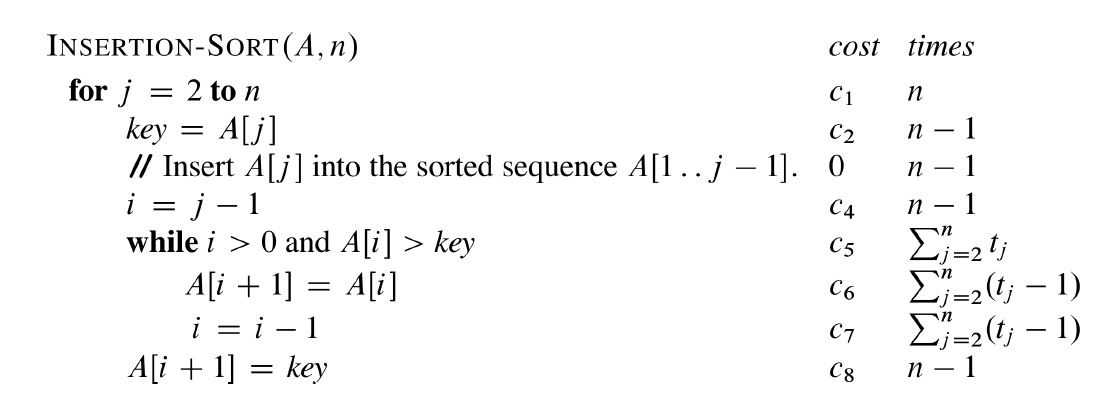
\includegraphics[width=0.9\linewidth]{insertion_sort.png}
    \end{figure}
    
    We are analyzing the time complexity of the \texttt{Insertion-Sort} algorithm. The cost of the algorithm is directly related to the number of times each step is repeated. Let’s go through the steps and calculate their costs.
    
    \subsection{Step-by-Step Cost Analysis}
    
    \begin{itemize}
        \item \textbf{Step 1:} The \texttt{for} loop iterates from $j = 2$ to $n$, so the condition is checked $n$ times, including the final check that fails. Hence, the total cost for this step is $c_1 \cdot n$.
        
        \item \textbf{Step 2:} The body of the \texttt{for} loop is executed $n-1$ times. Thus, this step has a cost of $c_2 \cdot (n-1)$.
        
        \item \textbf{Step 3:} The comment within the code is not executed, so its cost is $0$, even though it is "executed" $n-1$ times. Therefore, $c_3 = 0$.
        
        \item \textbf{Step 4:} The statement $i = j-1$ inside the \texttt{for} loop is executed $n-1$ times, hence the cost is $c_4 \cdot (n-1)$.
        
        \item \textbf{Step 5:} The \texttt{while} loop is nested inside the \texttt{for} loop. The cost depends on how many times the \texttt{while} loop is executed for each $j$, denoted as $t_j$. Therefore, the cost is the sum of $t_j$ from $j=2$ to $n$: 
        \[
        c_5 \cdot \sum_{j=2}^{n} t_j.
        \]
        
        \item \textbf{Steps 6 and 7:} The costs for these steps are also inside the \texttt{while} loop and depend on $t_j-1$, as the condition is not checked after the loop terminates. Hence, the total cost is:
        \[
        c_6 \cdot \sum_{j=2}^{n} (t_j - 1) + c_7 \cdot \sum_{j=2}^{n} (t_j - 1).
        \]
        
        \item \textbf{Step 8:} The assignment $A[i+1] = \texttt{key}$ occurs $n-1$ times, since it's inside the \texttt{for} loop. The total cost for this step is $c_8 \cdot (n-1)$.
    \end{itemize}
    
    \subsection{Overall Time Complexity}
    The total time complexity $T(n)$ of the \texttt{Insertion-Sort} algorithm is the sum of all these contributions:
    \[
    T(n) = c_1 \cdot n + c_2 \cdot (n-1) + 0 + c_4 \cdot (n-1) + c_5 \cdot \sum_{j=2}^{n} t_j + (c_6 + c_7) \cdot \sum_{j=2}^{n} (t_j - 1) + c_8 \cdot (n-1).
    \]
    
    \subsection{Best Case Scenario}
    In the best case, the input sequence is already sorted. This means that for all $j$, $t_j = 1$ (the \texttt{while} loop does not run). The time complexity becomes:
    \[
    T(n) = c_1 \cdot n + c_2 \cdot (n-1) + c_4 \cdot (n-1) + c_8 \cdot (n-1),
    \]
    which simplifies to:
    \[
    T(n) = (c_1 + c_2 + c_4 + c_8) \cdot n - (c_2 + c_4 + c_8).
    \]
    If we denote the constants as $b = c_1 + c_2 + c_4 + c_8$ and $d = -(c_2 + c_4 + c_8)$, the best case complexity is:
    \[
    T(n) = bn + d.
    \]
    In this case, everything inside the \texttt{while} loop is skipped and we assume all the constant equal to 1. Therefore, $T(n) = 5n - 4$.
    
    \subsection{Worst Case Scenario}
    In the worst case, the input sequence is sorted in reverse order. Here, $t_j = j$, which means the \texttt{while} loop executes $j$ times for $j=2,...,n$. The total cost for steps 5, 6, and 7 is:
    \[
    \sum_{j=2}^{n} t_j = \frac{n(n+1)}{2} - 1,
    \]
    and for steps 6 and 7:
    \[
    \sum_{j=2}^{n} (t_j - 1) = \frac{n(n-1)}{2}.
    \]
    Thus, the total time complexity in the worst case becomes:
    \[
    T(n) = c_1 \cdot n + c_2 \cdot (n-1) + c_4 \cdot (n-1) + c_5 \cdot \left(\frac{n(n+1)}{2} - 1\right) + (c_6 + c_7) \cdot \frac{n(n-1)}{2} + c_8 \cdot (n-1).
    \]
    This simplifies to:
    \[
    T(n) = \frac{3}{2}n^2 + \frac{7}{2}n - 4.
    \]
    
    \subsection{General Case}
    In general, the time complexity in the best case is $T(n) = bn + c$, where $b$ and $c$ are real constants, while in the worst case, it is $T(n) = an^2 + bn + c$, where $a$, $b$, and $c$ are real constants.

    \section{Selection Sort}
    Selection Sort is a simple comparison-based sorting algorithm that works by repeatedly selecting the smallest (or largest) element from an unsorted portion of the array and swapping it with the first unsorted element. 
    
    \subsection{Example}
    Consider the array \( A = [2, 5, 6, 4, 1, 3] \). The goal is to sort this array in ascending order using Selection Sort.
    
    \subsection{Steps of the Algorithm}
    \begin{itemize}
        \item Initial Setup: Start with the first element of the array as the current position \( j \) (initially \( j = 1 \)).
        \item Finding the Minimum: Compare the element at smallest with each subsequent element in the array:
        \begin{verbatim}
            For \( i = j + 1 \) to \( n \):
                If \( A[i] < A[smallest] \), update smallest to \( i \).
        \end{verbatim}
        \item Swap: After the inner loop completes, swap the elements at positions \( j \) and smallest.
        \item Repeat: Increment \( j \) and repeat the process until the entire array is sorted.
    \end{itemize}
    
    \subsection{Detailed Example Steps}
    \begin{itemize}
        \item Step 1: \begin{itemize}
            \item \( j = 1 \): \( A = [2, 5, 6, 4, 1, 3] \)
            \item Smallest is initially at index 1 (value 2).
            \item Compare with elements at indices 2 to 6.
            \item Smallest value found at index 5 (value 1).
            \item Swap \( A[1] \) with \( A[5] \):
            \item Result: \( A = [1, 5, 6, 4, 2, 3] \)
        \end{itemize}
        \item Step 2: \begin{itemize}
            \item \( j = 2 \): \( A = [1, 5, 6, 4, 2, 3] \)
            \item Smallest is at index 2 (value 5).
            \item Compare with elements at indices 3 to 6.
            \item Smallest value found at index 5 (value 2).
            \item Swap \( A[2] \) with \( A[5] \):
            \item Result: \( A = [1, 2, 6, 4, 5, 3] \)
        \end{itemize}
        \item Further Steps: Continue this process until \( j = n-1 \).
    \end{itemize}
    
    \subsection{Complexity Analysis}
    Selection Sort has a consistent time complexity of \( O(n^2) \), regardless of the initial order of the elements. This is because the algorithm always examines every element to find the minimum for each position in the array.
    
    There are no best-case or worst-case scenarios that can reduce the complexity since the algorithm must always perform the same number of comparisons.
    
    \subsection{Pseudocode}
    The pseudocode for Selection Sort is as follows:
    
    \begin{verbatim}
    n = length(A)
    for j = 1 to n - 1 do:
        smallest = j
        for i = j + 1 to n do:
            if A[i] < A[smallest] then
                smallest = i
        exchange A[j] with A[smallest]
    \end{verbatim}
    In Python, the exchange can be implemented using a temporary variable:
    \begin{verbatim}
    tmp = A[j]
    A[j] = A[smallest]
    A[smallest] = tmp
    \end{verbatim}
    
    \subsection{Cost Analysis}
    Let's denote the cost of each operation in the pseudocode:
    
    \begin{enumerate}
        \item Step 1 is executed once: \( 1 \)
        \item Step 2 is executed \( n \) times: \( n \)
        \item Step 3 is executed \( n-1 \) times: \( n - 1 \)
        \item Steps 4 and 5 are the sum of \( j \) from \( 1 \) to \( n-1 \): \( \sum_{j=1}^{n-1} t_j \)
        \item Steps 6 is the sum of \( j \) from \( 1 \) to \( n-1 \): \( 2 \sum_{j=1}^{n-1} (t_j - 1) \)
        \item Step 7 is executed \( n - 1 \) times: \( n - 1 \)
    \end{enumerate}
    The total cost \( T(n) \) in operations is given by:
    \[
    T(n) = 1 + n + (n - 1) + \sum_{j=1}^{n-1} t_j + 2 \sum_{j=1}^{n-1} (t_j - 1) + (n - 1)
    \]
    Using the steps for Insertion Sort, we can derive that:
    \[
    T(n) = 3n - 1 + \frac{n(n-1)}{2} + n(n-1) - 1
    \]
    Thus, the complexity of Selection Sort is in the order of \( O(n^2) \), it's remains the same for the best and worst case since we have to do the two for loops.
    
    \section{When to Use Selection Sort vs Insertion Sort}
    Selection Sort is generally not stable and does not perform well on large datasets due to its \( O(n^2) \) complexity. However, it has the advantage of performing a constant number of swaps, making it useful when memory writes are costly. \newline
    Insertion Sort, on the other hand, is more efficient for smaller datasets or partially sorted arrays, as it has a best-case time complexity of \( O(n) \) when the array is already sorted. Thus, Insertion Sort is preferable when dealing with nearly sorted data or small lists. In the best case Insertion sort is only $\Theta(n)$ since it doesn't enter the while loop.
    
\chapter{Random Variables: Absolutely Continuous and Singular Distributions}
    \chapter{Asymptotical Analysis}
    \section{Introduction to Asymptotic Analysis}
    
    Asymptotic analysis is used to describe the running time of an algorithm in terms of the input size \(n\) as \(n \rightarrow \infty\). It allows us to abstract away constants and focus on the growth of functions, comparing algorithms based on their efficiency. \newline    
    Let us consider two algorithms, \(A\) and \(B\), where the running time of algorithm \(A\), denoted as \(T_A(n) \sim n^2\), while for algorithm \(B\), the running time \(T_B(n) \sim n\). We can conclude that algorithm \(B\) is more efficient than algorithm \(A\) for all \(n \geq n_0\), where \(n_0\) is some sufficiently large threshold.
    
    \section{Asymptotic Notation}
    
    We use asymptotic notation to formalize this comparison. The goal is to describe the behavior of functions \(f(n)\) and \(g(n)\) as \(n\) becomes large. Consider the following types of asymptotic notation:
    
    \subsection{Big-Theta (\(\Theta\)) Notation}
    
    The function \(T_A(n)\) is said to be \(\Theta(g(n))\), denoted as:
    \[
    T_A(n) = \Theta(n^2)
    \]
    This means that \(T_A(n)\) is asymptotically bounded both above and below by \(g(n)\). Formally, 
    \[
    f(n) = \Theta(g(n))
    \] if there exist constants \(c_1, c_2 > 0\) and \(n_0 > 0\) such that:
    \[
    0 \leq c_1 g(n) \leq f(n) \leq c_2 g(n) \quad \text{for all} \quad n \geq n_0.
    \]
    In other words, \(f(n)\) lies between \(c_1 g(n)\) and \(c_2 g(n)\) for sufficiently large \(n\).
    
    \subsubsection{Example:}
    Let’s prove that \(f(n) = \frac{1}{2}n^2 - 3n\) is \(\Theta(n^2)\). \newline
    We need to find constants \(c_1, c_2 > 0\) and \(n_0 > 0\) such that:
    \[
    c_1 n^2 \leq \frac{1}{2}n^2 - 3n \leq c_2 n^2 \quad \text{for all} \quad n \geq n_0.
    \]
    1. Divide both sides by \(n^2\):
    \[
    c_1 \leq \frac{1}{2} - \frac{3}{n} \leq c_2.
    \]
    2. Choose \(n_0 = 7\), \(c_1 = \frac{1}{14}\), and \(c_2 = \frac{1}{2}\), ensuring that the inequality holds for all \(n \geq n_0\).
    
    \subsection{Big-O (\(O\)) Notation}
    
    Big-O notation defines an upper bound on the growth of a function, so provides an upper bound on the time taken by an algorithm in terms of the size of the input. For example, if \(T_B(n) = O(n)\), it means that \(T_B(n)\) grows at most as fast as \(n\). Formally, \(f(n) = O(g(n))\) if there exists a constant \(c > 0\) and \(n_0 > 0\) such that:
    \[
    0 \leq f(n) \leq c g(n) \quad \text{for all} \quad n \geq n_0.
    \] $\\$
    The \(f(n)\) function represents the number of operations (steps) that an algorithm performs to solve a problem of size n.
    
    \subsubsection{Example:}
    Let’s prove that \(f(n) = n + 4\) is \(O(n^2)\). \newline
    1. We need to find constants \(c > 0\) and \(n_0 > 0\) such that:
    \[
    f(n) \leq c n^2 \quad \text{for all} \quad n \geq n_0.
    \]
    2. We can choose \(c = 1\) and \(n_0 = 1\) to satisfy the inequality \(n + 4 \leq n^2\) for all \(n \geq n_0\).
    
    \subsection{Big-Omega (\(\Omega\)) Notation}
    
    Big-Omega notation provides a lower bound for the growth of a function. For example, \(T_A(n) = \Omega(n^2)\) means that \(T_A(n)\) grows at least as fast as \(n^2\). Formally, \(f(n) = \Omega(g(n))\) if there exists a constant \(c > 0\) and \(n_0 > 0\) such that:
    \[
    f(n) \geq c g(n) \quad \text{for all} \quad n \geq n_0.
    \]
    
    \subsubsection{Example:}
    Let’s prove that \(6n^3\) is not \(\Theta(n^2)\) by contradiction.
    \newline
    Assume that \(6n^3 = O(n^2)\), meaning there exists a constant \(c > 0\) such that:
    \[
    6n^3 \leq c n^2 \quad \text{for all} \quad n \geq n_0.
    \]
    Dividing both sides by \(n^2\), we get:
    \[
    6n \leq c.
    \]
    This leads to a contradiction because \(6n\) grows unbounded as \(n\) increases, while \(c\) is a constant.
    
    \section{General Polynomial Functions and Their Growth}
    
    For any polynomial function of degree \(d\), such as:
    \[
    f(n) = a_d n^d + a_{d-1} n^{d-1} + \cdots + a_1 n + a_0,
    \]
    we can say that \(f(n) = \Theta(n^d)\). The lower-order terms and constants do not affect the asymptotic growth, so:
    \[
    f(n) = \Theta(n^d).
    \]
    
    \section{Theorem: Relationship Between Asymptotic Notations}
    
    For any two functions \(f(n)\) and \(g(n)\):
    \[
    f(n) = \Theta(g(n)) \quad \text{if and only if} \quad f(n) = O(g(n)) \quad \text{and} \quad f(n) = \Omega(g(n)).
    \]
    This theorem implies that if \(f(n)\) is both \(O(g(n))\) and \(\Omega(g(n))\), it must also be \(\Theta(g(n))\).
    
    \subsubsection{Example:}
    Let’s prove that \(f(n) = (n + a)^b\) is \(O(n^b)\) for \(b \geq 0\). Divide both sides by \(n^b\), then simplify:
    \[
    \frac{(n+a)^b}{n^b} = \left( 1 + \frac{a}{n} \right)^b \leq 2,
    \]
    showing that \(f(n)\) is \(O(n^b)\).
    
    \subsection{Exponential Growth}
    
    Finally, consider an exponential function like \(f(n) = 2^{n+1}\). We want to show that \(f(n) = O(2^n)\). \newline 
    1. Start by simplifying \(2^{n+1}\):
    \[
    2^{n+1} = 2 \cdot 2^n.
    \]
    2. This shows that \(f(n) = O(2^n)\), where the constant \(c = 2\).

\chapter{Random Variables Distribution}
    \chapter{Divide and Conquer}

    \section{Recursive Algorithms}
    Before discussing divide-and-conquer algorithms, it is essential to understand the concept of recursive algorithms. A recursive algorithm is one that calls itself one or more times to solve a problem. The core idea is to divide the problem into smaller and simpler sub-problems, solve them individually, and then combine the solutions.
    
    A classical example is calculating the power of a number. For instance, calculating \(2^3\) can be done recursively by breaking it down as:
    \[
    2^3 = 2 \times 2^2 = 2 \times (2 \times 2^1)
    \]
    
    Recursion differs from iteration. While iteration involves loops, recursion involves a function calling itself. Iteration is generally more efficient in terms of constant factors, but recursion can simplify the design of an algorithm.
    
    \subsection{Base Case in Recursion}
    
    It is crucial that every recursive algorithm includes a base case, which provides a condition to stop the recursion. Without a base case, the algorithm would continue to call itself infinitely, leading to a stack overflow.
    
    \subsection{Execution Stack}
    Each time a recursive call is made, the current state of the function is saved in the execution stack (a LIFO structure). This is similar to a stack of objects where new items are added to the top. Once a function completes, its state is removed from the stack, and the previous function call is resumed. 
    
    For example, the execution stack for the function \texttt{RECURSIVE-POWER(2,3)} works as follows:
    
    \begin{itemize}
        \item The initial call \texttt{RECURSIVE-POWER(2,3)} leads to the call \texttt{RECURSIVE-POWER(2,2)}.
        \item Then, \texttt{RECURSIVE-POWER(2,2)} calls \texttt{RECURSIVE-POWER(2,1)}.
        \item Once \texttt{RECURSIVE-POWER(2,1)} returns the result, the previous calls are resumed until the final result is computed.
    \end{itemize}
    
    \section{Divide-and-Conquer Strategy}
    
    The divide-and-conquer strategy is commonly used in recursive algorithms. This strategy involves three main steps:
    \begin{itemize}
        \item \textbf{Divide:} Break the problem into smaller sub-problems.
        \item \textbf{Conquer:} Solve each sub-problem recursively.
        \item \textbf{Combine:} Combine the solutions of the sub-problems to form the final solution.
    \end{itemize}
    
    A classical example of this strategy is the \textbf{Merge-Sort} algorithm.
    
    \subsection{Merge-Sort Algorithm}
    
    Merge-sort is a sorting algorithm that follows the divide-and-conquer paradigm. Here are the steps:
    \begin{enumerate}
        \item Assume we have an unordered sequence of \(n\) elements.
        \item \textbf{Divide:} Split the sequence into two halves, each of length \(n/2\).
        \item \textbf{Conquer:} Sort both halves recursively using merge-sort.
        \item \textbf{Combine:} Merge the two sorted halves into one sorted sequence.
    \end{enumerate}
    
    The key part of the algorithm is the \textbf{combine} step, where two sorted arrays are merged.
    \begin{figure}[h!]
        \centering
        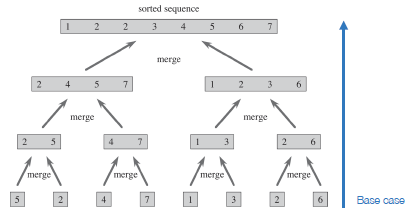
\includegraphics[width=0.75\linewidth]{immagini/merge_sort.png}
    \end{figure}
    \subsubsection{Merge-Sort Pseudo code}
    
    \begin{verbatim}
    MERGE-SORT(A, p, r)
        if p >= r
            return
        q = (p + r) / 2
        MERGE-SORT(A, p, q)
        MERGE-SORT(A, q+1, r)
        MERGE(A, p, q, r)
    \end{verbatim}
    
    Here, \(p\) and \(r\) represent the indices of the first and last elements of the array, and \(q\) is the middle index. The array is recursively split and sorted, and finally, the \texttt{MERGE} procedure combines the results.
    
    \subsubsection{Merge Procedure Pseudo code}
    
    \begin{verbatim}
    MERGE(A, p, q, r)
        n1 = q - p + 1
        n2 = r - q
        let L[1..n1+1] and R[1..n2+1] be new arrays
        for i = 1 to n1
            L[i] = A[p + i - 1]
        for j = 1 to n2
            R[j] = A[q + j]
        L[n1+1] = +infinite
        R[n2+1] = +infinite
        i = 1
        j = 1
        for k = p to r
            if L[i] <= R[j]
                A[k] = L[i]
                i = i + 1
            else
                A[k] = R[j]
                j = j + 1
    \end{verbatim}
    
    The \texttt{MERGE} function combines two sorted sub-arrays, \(L\) and \(R\), into a single sorted array. The use of sentinel values (\(\infty\)) ensures that the merging process can terminate correctly without additional checks.
    
    \section{Cost Analysis of Merge-Sort}
    The cost of Merge-Sort can be analyzed using recurrence relations. Here's the step-by-step breakdown:
    
    \subsection{Step 1: Divide the Array}
    
    Each time we divide the array, the size of the problem is halved. This results in two sub-problems of size \(n/2\). The time required to divide the array into two halves is constant, specifically \(\Theta(1)\), since it only involves calculating the midpoint \(q = (p + r) / 2\).
    
    \subsection{Step 2: Conquer the sub-problems}
    
    The two sub-problems are solved recursively, and the time to solve each sub-problem is given by the same merge-sort process. Therefore, the time required for solving both halves is \(T(n/2)\).
    
    \subsection{Step 3: Combine the Results (Merge Step)}
    
    The \texttt{MERGE} function takes \(\Theta(n)\) time because it processes all elements of the two sub-arrays, comparing and merging them into a single array. The merging process requires one pass through the elements, resulting in linear time complexity.
    
    \subsection{Overall Recurrence Relation}
    
    The time complexity of merge-sort can be described by the following recurrence relation:
    \[
    T(n) = 2T\left(\frac{n}{2}\right) + \Theta(n)
    \]
    This relation reflects the fact that we are solving two sub-problems of size \(n/2\), and the merging step takes \(\Theta(n)\) time.
    
    \subsection{Solving the Recurrence Relation}
    
    To solve this recurrence relation, we can use the \textbf{recursion tree method} or the \textbf{master theorem}. Let's go through the steps:
    \begin{enumerate}
        \item Recursive Expansion: Start by expanding the recurrence relation:
       \[
       T(n) = 2T\left(\frac{n}{2}\right) + \Theta(n)
       \]
       \[
       = 2\left(2T\left(\frac{n}{4}\right) + \Theta\left(\frac{n}{2}\right)\right) + \Theta(n)
       \]
       \[
       = 4T\left(\frac{n}{4}\right) + 2\Theta\left(\frac{n}{2}\right) + \Theta(n)
       \]
       \[
       = 8T\left(\frac{n}{8}\right) + 4\Theta\left(\frac{n}{4}\right) + 2\Theta\left(\frac{n}{2}\right) + \Theta(n)
       \]
       After expanding \(k\) times, we obtain:
       \[
       T(n) = 2^k T\left(\frac{n}{2^k}\right) + \sum_{i=0}^{k-1} 2^i \Theta\left(\frac{n}{2^i}\right)
       \] 
        \item Base Case:
       The base case occurs when the size of the sub-problem becomes 1, i.e., when \(n/2^k = 1\), which implies \(k = \log_2 n\). Substituting this into the expansion:
       \[
       T(n) = 2^{\log_2 n} T(1) + \sum_{i=0}^{\log_2 n - 1} 2^i \Theta\left(\frac{n}{2^i}\right)
       \]
       Since \(T(1)\) is a constant, we get:
       \[
       T(n) = n \cdot \Theta(1) + \sum_{i=0}^{\log_2 n - 1} \Theta(n)
       \]
        \item Sum Simplification:
       The sum simplifies to:
       \[
       \sum_{i=0}^{\log_2 n - 1} \Theta(n) = \log_2 n \cdot \Theta(n)
       \]
        \item Final Time Complexity:
       Therefore, the total time complexity is:
       \[
       T(n) = \Theta(n) + \log_2 n \cdot \Theta(n) = \Theta(n \log n)
       \]
    \end{enumerate}
        
    \subsection{Summary of Merge-Sort Complexity}
    
    Merge-Sort has a time complexity of \(\Theta(n \log n)\), which is optimal for comparison-based sorting algorithms. This time complexity holds for both the average and worst cases due to the divide-and-conquer structure, where the number of levels in the recursion tree is \(\log_2 n\), and each level performs \(\Theta(n)\) work for merging. The height of the tree is $h = log_2 n + 1$ and it has $n$ leaves.

\section{Recursion Tree Method for Complexity Analysis}

The recursion tree method is a visual tool to help analyze the complexity of recursive functions. Let’s consider the following exercises to explore this method in detail.

\subsection{Exercise 1: Analyzing \( T(n) = 3T\left(\frac{n}{4}\right) + \Theta(n^2) \)}
Given the recurrence relation:
\[
T(n) = 3T\left(\frac{n}{4}\right) + c n^2
\]
where \(c > 0\), \(a = 3\) is the number of subproblems, and \(b = 4\) represents the factor by which the problem size is reduced. The initial cost function \(cn^2\) is quadratic, meaning that the cost at each level will follow this quadratic pattern as the problem size decreases.

\subsection{Step-by-Step Analysis Using Recursion Tree}
\begin{enumerate}
    \item \textbf{Root Level}: At the root, the cost is \(cn^2\).

    \item \textbf{First Level of Subproblems}: We divide the problem into three subproblems, each of size \(n/4\), with cost:
   \[
   3 \cdot \left(\frac{n}{4}\right)^2 \cdot c = \frac{3}{16} n^2 c
   \]

    \item \textbf{Second Level}: Each subproblem of size \(n/4\) is divided again, resulting in three more subproblems per branch. The cost at this level becomes:
   \[
   \left(\frac{3}{16}\right)^2 n^2 c
   \]

    \item \textbf{Recursive Pattern}: We continue this process until reaching the leaves of the recursion tree, where the cost is constant (\(T(1)\)).
\end{enumerate}


\subsection{Calculating Total Cost}

The height of the tree is:
\[
h = \log_b n = \log_4 n
\]
and the number of leaves at the final level is approximately \(n\).

The total cost \(T(n)\) is the sum of the costs across each level:
\[
T(n) = \sum_{i=0}^{\log_4 n - 1} \left(\frac{3}{16}\right)^i \cdot c \, n^2 + \Theta(n^{\log_4 3})
\]

We can approximate this sum with an infinite geometric series:
\[
T(n) < \sum_{i=0}^{\infty} \left(\frac{3}{16}\right)^i \cdot c \, n^2
\]

Using the formula for the sum of an infinite geometric series \(\sum_{k=0}^{\infty} x^k = \frac{1}{1-x}\) for \(|x| < 1\), we get:
\[
T(n) < \frac{1}{1 - \frac{3}{16}} \cdot c \, n^2 + \Theta(n^{\log_4 3}) = \frac{16}{13} c \, n^2 + \Theta(n^{\log_4 3})
\]
Thus, we conclude:
\[
T(n) = O(n^2)
\]

\begin{center}
    \textbf{Recursion Tree for \(T(n) = 3T\left(\frac{n}{4}\right) + \Theta(n^2)\)}
\end{center}

\begin{tikzpicture}
    [level distance=1.5cm, sibling distance=4cm, edge from parent/.style={draw,-latex}]
    \node { \( T(n) = cn^2 \) }
        child { node { \( T(n/4) = \frac{3}{16} cn^2 \) }
            child { node { \( T(n/16) = \left(\frac{3}{16}\right)^2 cn^2 \) } }
            child { node { \( T(n/16) = \left(\frac{3}{16}\right)^2 cn^2 \) } }
            child { node { \( T(n/16) = \left(\frac{3}{16}\right)^2 cn^2 \) } }
        }
        child { node { \( T(n/4) = \frac{3}{16} cn^2 \) } }
        child { node { \( T(n/4) = \frac{3}{16} cn^2 \) } };
\end{tikzpicture}

\subsection{Exercise 2: Analyzing \( T(n) = T\left(\frac{n}{3}\right) + T\left(\frac{2n}{3}\right) + cn \)}

Given the recurrence relation:
\[
T(n) = T\left(\frac{n}{3}\right) + T\left(\frac{2n}{3}\right) + cn
\]
\begin{enumerate}
    \item Root Level: At the root, the cost is \(cn\).
    \item Division into Subproblems: We divide the problem into subproblems of size \(n/3\) and \(2n/3\), each with cost proportional to \(cn\). 
    \item Continuing the Division: This is an unbalanced tree, as the \(2n/3\) branch will continue dividing for more levels than the \(n/3\) branch.
\end{enumerate}

Since the right branch (\(2n/3\)) divides more slowly, it will dominate the total cost. Therefore, we approximate the cost by following the longer branch.

\subsection{Calculating Height and Total Cost}

The height \(h\) of the tree based on the \(2n/3\) branch is:
\[
h = \log_{3/2} n
\]
Since each level has a cost \(cn\), the total cost is:
\[
T(n) = cn \cdot \log_{3/2} n = O(n \log n)
\]

\begin{center}
    \textbf{Partial Recursion Tree for \(T(n) = T\left(\frac{n}{3}\right) + T\left(\frac{2n}{3}\right) + cn\)}


\begin{tikzpicture}
    [level distance=1.5cm, sibling distance=3cm, edge from parent/.style={draw,-latex}]
    \node { \( T(n) = cn \) }
        child { node { \( T(n/3) = \frac{1}{3} cn \) } }
        child { node { \( T(2n/3) = \frac{2}{3} cn \) }
            child { node { \( T(2n/9) = \frac{2}{9} cn \) }
                child { node { \(\cdots\) } }
            }
            child { node { \( T(4n/9) = \frac{4}{9} cn \) }
                child { node { \(\cdots\) } }
            }
        };
\end{tikzpicture}
\end{center}
\subsection{Summary}

In general, for a recurrence relation \( T(n) = a T\left(\frac{n}{b}\right) + \Theta(n^\alpha) \):
\begin{itemize}
    \item The recursion tree height is \( h = \log_b n \).
    \item The cost at each level is determined by the number of subproblems \(a\), the size reduction factor \(b\), and the initial complexity \(\alpha\).
    \item The total cost is derived from the sum of work at each level, up to the leaves.
\end{itemize}

\section{Exercise: Algorithm with Complexity \(\Theta(n \log n)\)}

Given a set \(S\) of \(n\) integers and another integer \(X\), determine if there exists a pair of elements in \(S\) whose sum equals \(X\). Note that we only need to find one such pair if it exists; it does not matter which pair.

A straightforward brute-force approach would involve two nested loops: for each element \(y \in S\), check if there exists another element \(w \in S\) such that \(y + w = X\). However, this approach has a time complexity of \(\Theta(n^2)\), which is suboptimal.

\subsection{Optimized Approach}
We aim to achieve a time complexity of \(\Theta(n \log n)\). Since sorting algorithms like merge-sort have this complexity, we can leverage sorting in our solution.

If there exist elements \(y, w \in S\) such that \(y + w = X\), then:
\[
w = X - y
\]
Define a new set \(S'\) as follows:
\[
            S' = \{z = X - y \mid y \in S\}
            \]
\begin{itemize}
    \item Sort \(S\) and \(S'\) using merge-sort, each with a time complexity of \(\Theta(n \log n)\).
    \item Merge \(S\) and \(S'\) into a new sequence \(S''\).
    \item Check if there exists an element in \(S\) that appears in \(S''\).
\end{itemize}

\subsection{Complexity Analysis}
\begin{itemize}
    \item Creating \(S'\) has a linear cost: \(\Theta(n)\).
    \item Sorting \(S\) and \(S'\) requires \(\Theta(n \log n)\).
    \item Merging \(S\) and \(S'\) takes linear time: \(\Theta(n)\).
    \item Checking for duplicate elements in \(S''\) also has a linear cost: \(\Theta(n)\).
\end{itemize}

Therefore, the total time complexity is:
\[
\Theta(n) + 2 \Theta(n \log n) = \Theta(n \log n)
\]

\section{Exercise: Finding an Element in a Sequence}

Given a sequence \(S\) of integers and an integer \(X\), determine whether \(X \in S\) and return the index \(i\) such that \(S[i] = X\).

\subsection{Linear Search}
If \(S\) is unordered, we must scan the entire sequence, resulting in a time complexity of \(\Theta(n)\). This is known as the linear scan.

\subsection{Binary Search}
If \(S\) is ordered, we can use binary search, which divides the search interval in half each step:
\begin{enumerate}
    \item Define two indices, \( \text{low} \) and \( \text{high} \).
    \item  Compute the midpoint as:
   \[
   \text{mid} = \left\lfloor \frac{\text{high} + \text{low}}{2} \right\rfloor
   \]
    \item If \(X < S[\text{mid}]\), continue searching in the left half \([ \text{low}, \text{mid} - 1 ]\).
    \item If \(X > S[\text{mid}]\), search in the right half \([ \text{mid} + 1, \text{high} ]\).
    \item If \(X = S[\text{mid}]\), return \(\text{mid}\).
\end{enumerate}
Each division reduces the search space by half, leading to a logarithmic time complexity: \(\Theta(\log n)\), which matches the height of a binary tree.

\subsection{Iterative Binary Search Algorithm}

\begin{verbatim}
def iterative_binary_search(S, X, low, high):
    while low <= high:
        mid = (high + low) // 2  # Equivalent to the floor of (high + low) / 2
        if S[mid] == X:
            return mid
        elif S[mid] < X:
            low = mid + 1
        else:
            high = mid - 1
    return None  # Return None if X is not found
\end{verbatim}

The \texttt{None} return indicates that the element was not found.

\subsection{Complexity Analysis}
The recurrence relation for the binary search is:
\[
T(n) = T\left(\frac{n}{2}\right) + \Theta(1)
\]
since each iteration reduces the problem size by half with a constant operation. Solving this recurrence, we find:
\[
T(n) = \Theta(\log n)
\]

\newpage
   
\chapter{Notorious Random Variables}
    \chapter{Strassen Matrix Multiplication}
    
    Before introducing Strassen's method, let's examine standard matrix multiplication, called \textbf{Square-Matrix-Multiplication (SMMR)}. Given two \(n \times n\) matrices \(A\) and \(B\), we want to compute their product \(C = A \times B\).
    
    \subsection{Standard Matrix Multiplication (SMMR)}
    1. Divide matrices \(A\) and \(B\) as follows:
       \[
       A = \begin{bmatrix} A_{11} & A_{12} \\ A_{21} & A_{22} \end{bmatrix}, \quad B = \begin{bmatrix} B_{11} & B_{12} \\ B_{21} & B_{22} \end{bmatrix}
       \]
       
    2. Each element of \(C\) is computed as:
       \[
       C = A \times B = \begin{bmatrix} C_{11} & C_{12} \\ C_{21} & C_{22} \end{bmatrix}
       \]
       where
       \[
       C_{11} = A_{11} B_{11} + A_{12} B_{21}, \quad C_{12} = A_{11} B_{12} + A_{12} B_{22}
       \]
       \[
       C_{21} = A_{21} B_{11} + A_{22} B_{21}, \quad C_{22} = A_{21} B_{12} + A_{22} B_{22}
       \]
    
    This method requires 8 recursive multiplications for each submatrix.
    
    \subsection{Recursive SMMR Algorithm}
    
    \begin{verbatim}
    def SMMR(A, B):
        n = len(A)  # Number of rows in A
        C = [[0] * n for _ in range(n)]  # Initialize nxn matrix C with zeros
        
        if n == 1:
            C[0][0] = A[0][0] * B[0][0]
        else:
            # Partition matrices A, B, and C as described
            C11 = SMMR(A11, B11) + SMMR(A12, B21)
            C12 = SMMR(A11, B12) + SMMR(A12, B22)
            C21 = SMMR(A21, B11) + SMMR(A22, B21)
            C22 = SMMR(A21, B12) + SMMR(A22, B22)
            
            # Combine results into matrix C (requires additional merging steps in practice)
        
        return C
    \end{verbatim}
    
    \subsection{Complexity Analysis of SMMR}
    
    Dividing each matrix into four \( \frac{n}{2} \times \frac{n}{2} \) submatrices requires 8 multiplications. Assuming each submatrix has \( \left(\frac{n}{2}\right)^2 = \frac{n^2}{4} \) entries, we derive the recurrence:
    \[
    T(n) = \begin{cases} 
          \Theta(1) & \text{if } n = 1 \\
          8T\left(\frac{n}{2}\right) + \Theta(n^2) & \text{if } n > 1 
       \end{cases}
    \]
    
    The height of the recursion tree is \(\log_2 n\), and the total number of leaves is \(n^{\log_2 8} = n^3\), leading to:
    
    
    \section{Strassen's Algorithm}
    
    Strassen's algorithm presents a clever approach to improve the efficiency of matrix multiplication, specifically for large matrices. Although it is challenging to apply this algorithm beyond the context of matrix multiplication, studying it is highly useful for understanding the principles of recursion and complexity analysis in algorithms. 
    
    \subsection{Standard Recursive Matrix Multiplication}
    As previously discussed, multiplying two matrices \(A\) and \(B\) can be formulated as a recursive problem. Each matrix is divided into four \( \frac{n}{2} \times \frac{n}{2} \) submatrices, and recursive calls are made until we reach matrices of size \(1 \times 1\), where the multiplications are performed directly. This standard approach yields a time complexity of \(\Theta(n^3)\).
    
    \subsection{Overview of Strassen's Algorithm}
    Strassen’s algorithm reduces the complexity of matrix multiplication by leveraging specific combinations of additions and multiplications. It consists of four main steps:
    \begin{enumerate}
        \item Divide matrices \(A\) and \(B\) into \( \frac{n}{2} \times \frac{n}{2} \) submatrices, similar to the standard approach.
        \item Construct 10 intermediate matrices \( S_1, S_2, \dots, S_{10} \) of size \( \frac{n}{2} \times \frac{n}{2} \), each representing specific sums or differences of the submatrices of \(A\) and \(B\). These combinations are carefully chosen to optimize the calculation process, as we will see shortly. This step has a complexity of \(\Theta(n^2)\).
        \item Using the submatrices from steps 1 and 2, compute 7 product matrices \( P_1, P_2, \dots, P_7 \), each of size \( \frac{n}{2} \times \frac{n}{2} \), by recursively applying the Strassen algorithm.
        \item Finally, construct the resulting submatrices \( C_{11}, C_{12}, C_{21}, C_{22} \) for the product matrix \(C\), using the product matrices \(P_i\). This step also has a complexity of \(\Theta(n^2)\).
    \end{enumerate}
    
    The key improvement in Strassen's algorithm lies in reducing the number of recursive multiplications from 8 to 7, which reduces the overall complexity.
    
    \subsection{Detailed Steps of Strassen’s Algorithm}
    \subsubsection*{Step 1: Divide Matrices}
    This step involves partitioning \(A\) and \(B\) as:
    \[
    A = \begin{bmatrix} A_{11} & A_{12} \\ A_{21} & A_{22} \end{bmatrix}, \quad B = \begin{bmatrix} B_{11} & B_{12} \\ B_{21} & B_{22} \end{bmatrix}
    \]
    
    \subsubsection*{Step 2: Construct Intermediate Sum Matrices}
    Define the following intermediate matrices:
    \[
    \begin{aligned}
        S_1 &= B_{12} - B_{22}, \\
        S_2 &= A_{11} + A_{12}, \\
        S_3 &= A_{21} + A_{22}, \\
        S_4 &= B_{21} - B_{11}, \\
        S_5 &= A_{11} + A_{22}, \\
        S_6 &= B_{11} + B_{22}, \\
        S_7 &= A_{12} - A_{22}, \\
        S_8 &= B_{21} + B_{22}, \\
        S_9 &= A_{11} - A_{21}, \\
        S_{10} &= B_{11} + B_{12}.
    \end{aligned}
    \]
    
    \subsubsection*{Step 3: Compute Product Matrices}
    Calculate the seven product matrices as follows:
    \[
    \begin{aligned}
        P_1 &= A_{11} \cdot S_1, \\
        P_2 &= S_2 \cdot B_{22}, \\
        P_3 &= S_3 \cdot B_{11}, \\
        P_4 &= A_{22} \cdot S_4, \\
        P_5 &= S_5 \cdot S_6, \\
        P_6 &= S_7 \cdot S_8, \\
        P_7 &= S_9 \cdot S_{10}.
    \end{aligned}
    \]
    
    \subsubsection*{Step 4: Construct Final Product Matrix \(C\)}
    Using the product matrices \(P_1, P_2, \dots, P_7\), construct the final submatrices of \(C\):
    \[
    \begin{aligned}
        C_{11} &= P_5 + P_4 - P_2 + P_6, \\
        C_{12} &= P_1 + P_2, \\
        C_{21} &= P_3 + P_4, \\
        C_{22} &= P_5 + P_1 - P_3 - P_7.
    \end{aligned}
    \]
    The final product matrix \(C\) is given by:
    \[
    C = \begin{bmatrix} C_{11} & C_{12} \\ C_{21} & C_{22} \end{bmatrix}
    \]
    
    \subsection{Complexity Analysis of Strassen's Algorithm}
    Despite the algorithm's complexity in terms of individual operations, it reduces the number of multiplications needed, which decreases the overall complexity. Strassen's algorithm achieves a time complexity of:
    \[
    \Theta(n^{\log_2 7}) \approx \Theta(n^{2.8073})
    \]
    This represents a significant improvement over the standard matrix multiplication complexity of \(\Theta(n^3)\).

\chapter{Moment Generating Function and Characteristic Function}
    \chapter{Data Structure}

    In programming, we encounter various data structures beyond what is available in languages like Python. In Python, we often use lists to perform a variety of operations such as \texttt{pop}, \texttt{add}, \texttt{remove}, and \texttt{concatenate}, without explicit concerns about list size. Additionally, Python allows flexible data typing (e.g., adding an integer to a float), making it a convenient but less controlled environment. 
    
    \section{Data Types}
    A \textbf{data type} specifies the nature of values and defines the operations allowed on those values. For instance, in Python, stacks, queues, deques, and linked lists are often managed under the umbrella of lists, which provides flexibility but less control.
    
    \section{List}
    A \textbf{list} is a sequential collection of values, where each element has a specific position (or index).
    Indexes range from 0 to n-1( there n is the length of the list) or from 1 to n. Lists in Python are heterogeneous, meaning they can store values of different types, whereas strings are homogeneous since their elements are characters.
    
    Python supports several operations on lists, each of which is an example of an Abstract Data Type (ADT):
    \begin{itemize}
        \item \texttt{list.append(x)}: Add an item to the end of the list.
        \item \texttt{list.extend(L)}: Extend the list by appending all items in the given list \(L\).
        \item \texttt{list.insert(i, x)}: Insert item \(x\) at position \(i\).The first argument is the index of the element before which to insert, so a.insert(0,x) inserts at the front of the list.
        \item \texttt{list.remove(x)}:Remove the first item from the list whose value is x. It is an error if there is no such item.
        \item \texttt{list.pop(i)}: Remove and return the item at position \(i\), if no index is specified, a.pop() removes and returns the last item in the list.
        \item \texttt{list.index(x)}: Return the index of the first item  whose value is \(x\).
        \item \texttt{list.count(x)}: Count occurrences of \(x\) in the list.
    \end{itemize}
    
    \section{Stack}
    A \textbf{stack} is a collection of objects following the Last-In-First-Out (LIFO) principle, where elements are added to the top and removed from the top. The height (length) of the stack refers to the number of elements, while the top represents the most recently added element.
    
    Stack ADT(Abstract Data Type):
    \begin{itemize}
        \item \texttt{S.push(e)}: Add element \(e\) to the top.
        \item \texttt{S.pop()}: Remove and return the top element.
        \item \texttt{S.top()}: Return the top element without removing it.
        \item \texttt{S.is\_empty()}: Check if the stack is empty.
        \item \texttt{len(S)}: Return the length of the stack.
    \end{itemize}
    
    \section{Queue}
    A \textbf{queue} is a collection of objects following the First-In-First-Out (FIFO) principle, where elements are added at the back and removed from the front.
    
    Queue ADT:
    \begin{itemize}
        \item \texttt{Q.enqueue(e)}: Add element \(e\) to the back of the queue.
        \item \texttt{Q.dequeue()}: Remove and return the front element.
        \item \texttt{Q.first()}: Return the front element without removing it.
        \item \texttt{Q.is\_empty()}: Check if the queue is empty.
        \item \texttt{len(Q)}: Return the length of the queue.
    \end{itemize}
    
    \section{Deque}
    A \textbf{deque} (double-ended queue) it's a queue where you can get the first() or the last() element and allows elements to be added or removed from both ends. Unlike lists, deques restrict access to middle elements.
    
    Deque ADT:
    \begin{itemize}
        \item \texttt{Q.add\_first(e)}: Add element \(e\) to the front.
        \item \texttt{Q.add\_last(e)}: Add element \(e\) to the back.
        \item \texttt{Q.delete\_first()}: Remove and return the front element.
        \item \texttt{Q.delete\_last()}: Remove and return the back element.
        \item \texttt{Q.first()}, \texttt{Q.last()}, \texttt{Q.is\_empty()}, \texttt{len(Q)}: Same as queue operations.
    \end{itemize}
    
    In Python, deques can be implemented using the \texttt{collections} module. For example, \texttt{append()} adds to the back, and \texttt{popleft()} removes from the front.Given a deque D in Python, you can get an element at index i as D[i]. Indexed access is \(O(1)\) at both ends but degrades to \(O(n)\) for elements in the middle.
    
    \section{Linked List}
    A \textbf{linked list} is a data structure where elements are stored in nodes linked together in a sequence by pointers. Unlike arrays, where the order is maintained by indexes, linked lists maintain order through pointers.
    
    \subsection{Singly Linked List}
    In a singly linked list, each node has a value and a pointer to the next node. The first node is the head, and the last node is the tail. Maintaining a pointer to the head is essential for accessing the list. Traversing a list means moving from the head to the tail. A Linked List must maintain a pointer to the head, otherwise there is no way to locate that node. Sometimes also a pointed to the tail is stored (to avoid traversal). List “nodes” are “objects”.

    

    \begin{figure}[H]
        \centering
        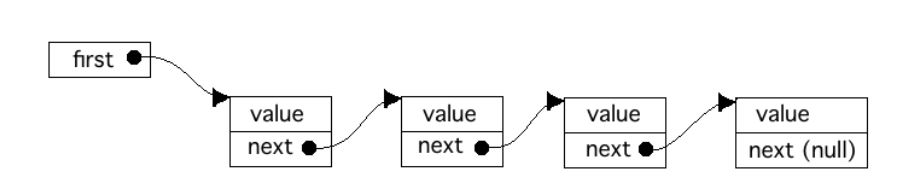
\includegraphics[width=0.5\linewidth]{immagini/singly linked list.JPG}
        \label{fig:enter-label}
    \end{figure}

    
    Adding a Node to a linked list
    \begin{enumerate}
        \item Create a new node, \texttt{newest = Node(e)}.
        \item Set \texttt{newest.next} to the current head:  \texttt{newest.next = L.head}
        \item Update \texttt{L.head} to point to \texttt{newest}.
        \item Increase the list size: \texttt{L.size=L.size+1}
    \end{enumerate}
    \begin{figure}[h!]
        \centering
        \begin{minipage}{0.45\textwidth}
          \centering
          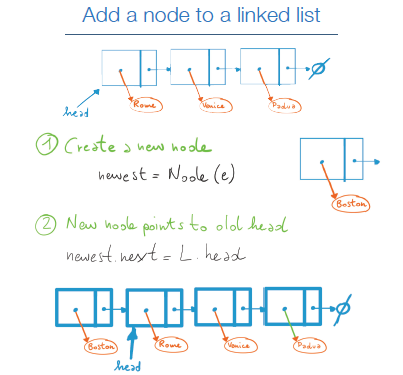
\includegraphics[width=\textwidth]{immagini/linkl1.png}
        \end{minipage}
        \hfill
        \begin{minipage}{0.45\textwidth}
          \centering
          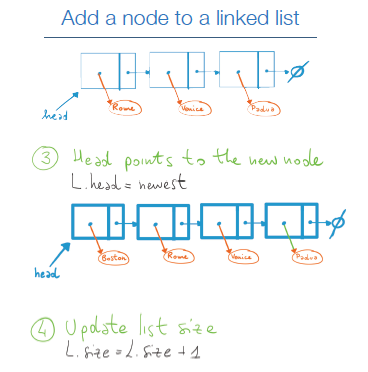
\includegraphics[width=\textwidth]{immagini/linkl2.png}
        \end{minipage}
        \label{fig:two_images}
    \end{figure}
    \newpage
    Removing a Node
    \begin{enumerate}
        \item Find the node with the value to remove (e.g., "Rome").
        \item Set \texttt{previous.next} to \texttt{current.next} and delete the current node.
    \end{enumerate}
    \begin{figure}[h!]
        \centering
        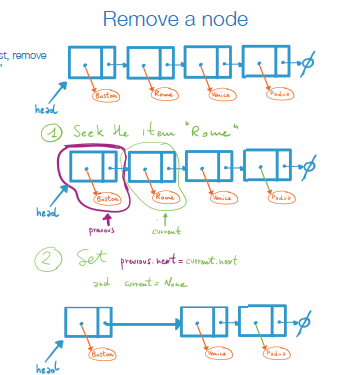
\includegraphics[width=0.5\linewidth]{immagini/linkl3.png}
    \end{figure}

    \subsection{Circularly Linked List}
    In a circularly linked list, the last node points back to the head, creating a circular structure. Be cautious with traversals as they loop infinitely.
    \begin{figure}[h]
        \centering
        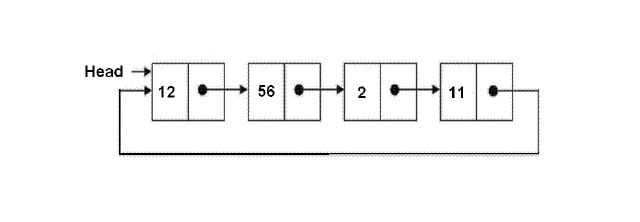
\includegraphics[width=0.8\linewidth]{immagini/circularly linked lists.JPG }
        \label{fig:enter-label}
    \end{figure}
    \newpage
    \subsection{Doubly Linked List}
    A doubly linked list has pointers in both directions, allowing traversal from both ends. It includes header and trailer nodes as sentinels, which simplify insertions.
    \begin{figure}[h!]
        \centering
        \begin{minipage}{0.7\textwidth}
          \centering
          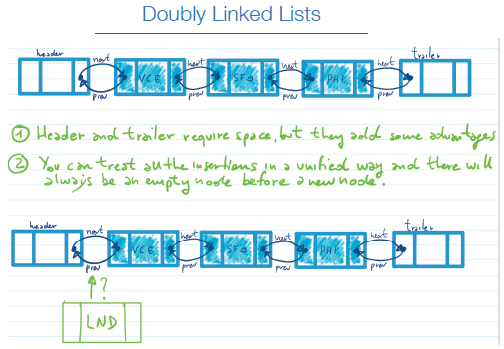
\includegraphics[width=\textwidth]{immagini/dlink1.png}
        \end{minipage}
        \hfill
        \begin{minipage}{0.7\textwidth}
          \centering
          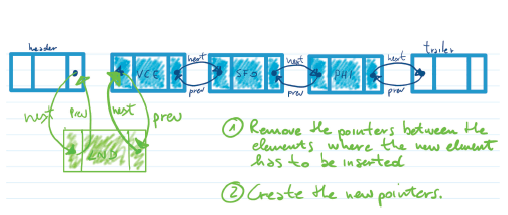
\includegraphics[width=\textwidth]{immagini/dlink2.png}
        \end{minipage}
        \label{fig:two_images}
    \end{figure}
    \subsection{Exercise: Find the Middle Node}
    Given a singly linked list of \(N\) nodes, find the middle node. If \(N\) is even, return the second middle element.
    
    \begin{itemize}
        \item Solution 1: Traverse the list and count nodes. Traverse again up to count/2 to find the middle node.
        \item Solution 2: Use two pointers, one moving twice as fast as the other. When the fast pointer reaches the end, the slow pointer is at the middle.
    \end{itemize}
    
    \subsection{Exercise: Check if a Linked List is a Palindrome}
    Given a singly linked list, check if it is a palindrome.
    
    \textbf{Solution}: Traverse the list, pushing each node onto a stack. Traverse again, popping elements from the stack and comparing each with the current node. If all match, return true.
    
    \subsection{Exercise: Reverse a Linked List}
    Given the head of a linked list, reverse the list.
    
    \textbf{Solution}:
    \begin{verbatim}
    current = head
    while current is not None:
        next = current.next
        current.next = prev
        prev = current
        current = next
    head = prev
    \end{verbatim}
    
    \subsection{Positional List}
    It is a data structure that allows us to perform arbitrary insertions and deletions or to refer to elements anywhere in a list. Numerical indexes are good, but they require to scan the entire list to find a specific element and to change dynamically when we update a list. An index does not always refer to the same element within a list. A positional list is an abstraction that provides the ability to identify the position of an element in a list.
    

    
    \section{Array vs. List-Based Data Structures}
    The complexity of those structure is different:
    \begin{itemize}
        \item Arrays: O(1)-time access to an element based on an index
        \item O(n) in a linked list to do the traversal
    \end{itemize}
    Also the storing consumption is different:
    \begin{itemize}
        \item Arrays: we may need to store 2n elements (dynamic resizing)
        \item Lists: we store n elements and n references (singly linked lists) and 2n references (doubly linked lists)
    \end{itemize}
    
    \begin{figure}[h]
        \centering
        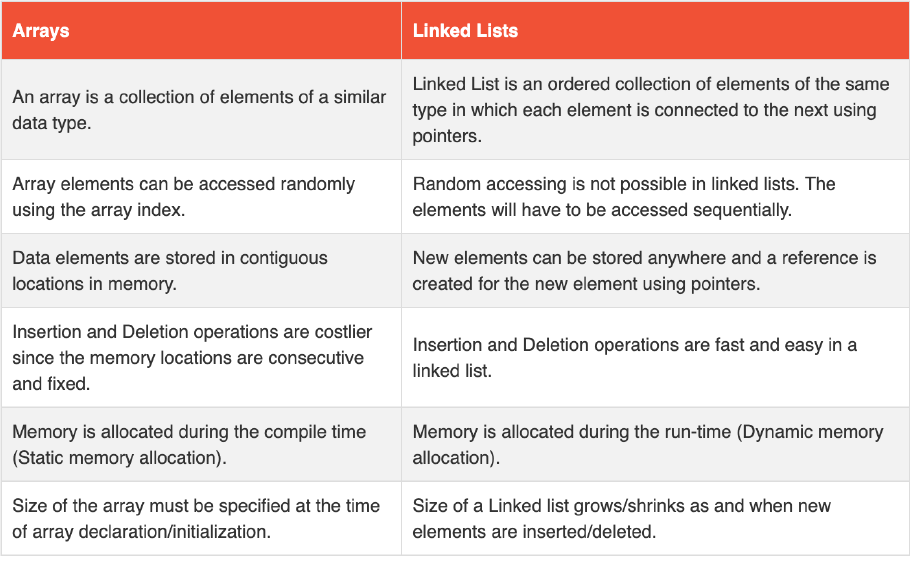
\includegraphics[width=0.9\linewidth]{immagini/06_data structure table .png}

    \end{figure}
        
    \section{Implementing Linked Lists with Arrays}

    \begin{enumerate}
        \item  Using Three Arrays: Implementation with three arrays:
                   \begin{itemize}
                       \item \texttt{next} keep the pointers to the next element.
                       \item \texttt{key} contains the actual elements.
                       \item \texttt{prev} stores the index of the previous element.
                   \end{itemize}
                Here, \texttt{L} maintains the index of the head.
        \item Using a Single Array: Represent objects in a contiguous sub-array \([j \dots k]\). Each attribute corresponds to an offset (e.g., key, next, prev), and the object's pointer is the starting index \(j\).
    \end{enumerate}
    \begin{figure}
        \centering
        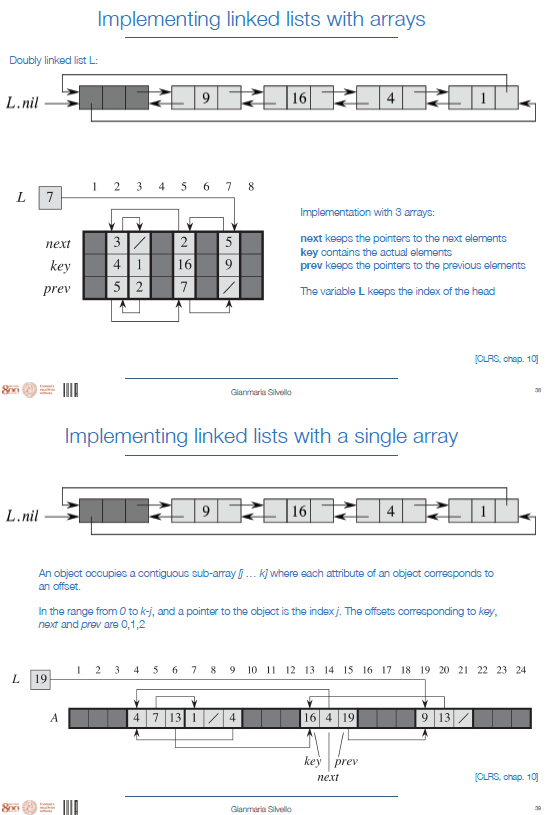
\includegraphics[width=1\linewidth]{immagini/listarray.png}
        \label{fig:enter-label}
    \end{figure}
    
    

    
    


\chapter{Convergence in Probability Theory}
    \chapter{Trees}

\section{Introduction to Trees}
\begin{figure}[h!]
    \centering
    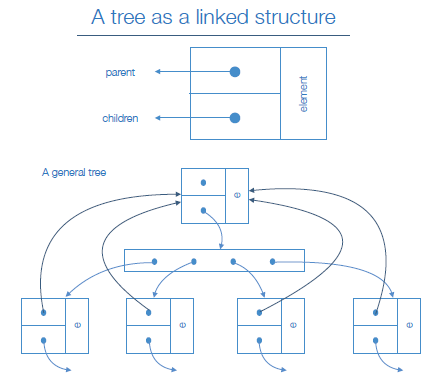
\includegraphics[width=0.75\linewidth]{immagini/general tree.png}
    \label{fig:enter-label}
\end{figure}
A \textbf{tree} is a data structure widely used to represent hierarchical relationships. It consists of nodes connected by edges and is fundamental in computer science for its structural properties. A formal tree structure satisfies the following conditions:
\begin{enumerate}
    \item It has \( n \) vertices and \( n - 1 \) edges.
    \item It is a connected graph without circuits.
    \item Any pair of vertices is connected by a unique path.
\end{enumerate}
If any of the above is true, the structure is a tree.

\section{Free Trees}
A \textbf{free tree} is a connected, acyclic, undirected graph. If a graph is acyclic but disconnected, it is termed a \textbf{forest}. Given an undirected graph \( G = (V, E) \):
\begin{itemize}
    \item If \( G \) is a free tree, any two vertices are connected by a unique path.
    \item \( G \) is connected, but if any edge is removed, the graph becomes disconnected.
    \item \( G \) has \( |E| = |V| - 1 \).
    \item \( G \) is acyclic, but adding any edge creates a cycle.
\end{itemize}

\section{Rooted Trees}
A \textbf{rooted tree} is a free tree where one of the nodes is called root.

    
\begin{figure}[h]
        \centering
        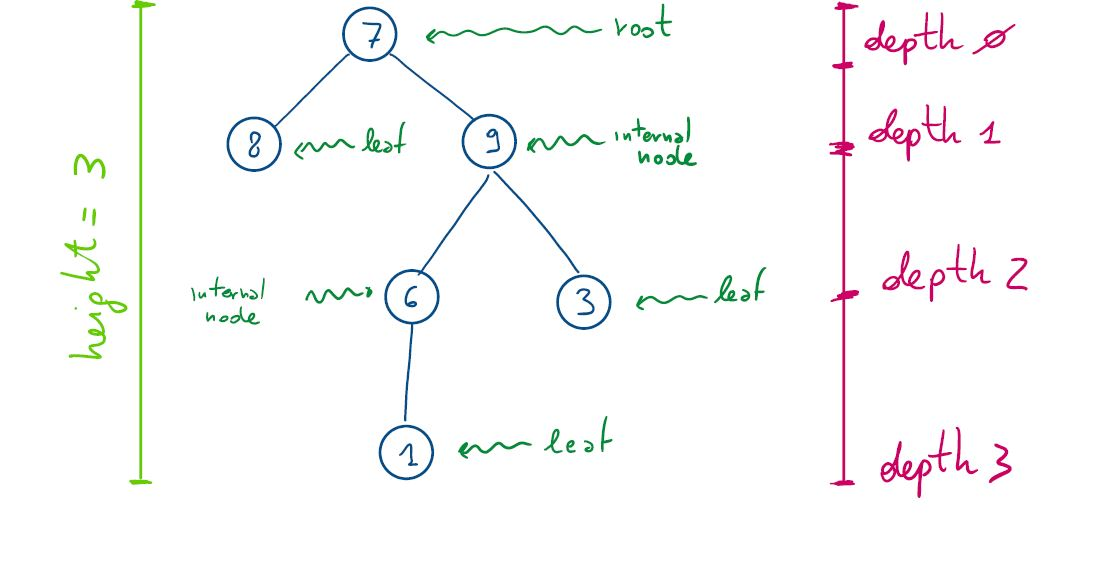
\includegraphics[width=0.5\linewidth]{immagini/rooated tree.JPG}
    \end{figure}



Each node in a rooted tree has:
\begin{itemize}
    \item \textbf{Parent}: The node directly linked above.
    \item \textbf{Child}: A node connected below.
    \item \textbf{Leaf}: A node with no children.
    \item \textbf{Internal node}: A node with at least one child.
    \item \textbf{Depth}: The level of a node from the root.
    \item \textbf{Degree}: The number of children of a node.
\end{itemize}

\subsection{Subtree and Ordered Trees}
The \textbf{subtree} rooted at \( x \) consists of \( x \) and all its descendants. In an \textbf{ordered tree}, the children of each node are arranged in a specific order (e.g.,if x has 3 children, say {y, w, z} we can say that y is the first child, w is the second child…).

\section{General Tree ADT}
The general tree Abstract Data Type (ADT) includes operations such as:
\begin{itemize}
    \item \texttt{p.element()}: Returns the element stored at position \( p \).
    \item \texttt{T.root()}: Returns the root of the tree or \texttt{None} if empty.
    \item \texttt{T.is\_root(p)}: Returns \texttt{True} if the node stored at position \( p \) is the root.
    \item \texttt{T.parent(p)}:Return the position of the parent of the node stored in \( p \).
    \item \texttt{T.num\_children(p)}: Returns the number of children of \( p \).
    \item \texttt{T.children(p)}: Generate an iteration of the children of position \( p \).
    \item \texttt{T.is\_leaf(p)} or \texttt{T.is\_external(p)}: Returns \texttt{True} if \( p \) is a leaf.
    \item \texttt{len(T)}: Returns the number of nodes.
    \item \texttt{T.is\_empty()}: Returns \texttt{True} if the tree is empty.
\end{itemize}

\section{Depth and Height of Trees}
\textbf{Depth} of a node \( p \) is the distance from \( p \) to the root. The \textbf{height} of a tree is the maximum depth among all nodes.

\subsection{Depth Calculation}
The depth of node \( p \) can be calculated using:
\begin{enumerate}
    \item Recursive method:
    \begin{verbatim}
    depth(T, p):
        if T.is_root(p):
            return 0
        else:
            return 1 + depth(T, T.parent(p))
    \end{verbatim}
    \item Iterative method:
    \begin{verbatim}
    depth(T, p):
        d = 0
        while T.parent(p) is not None:
            d += 1
            p = T.parent(p)
        return d
    \end{verbatim}
\end{enumerate}

\subsection{Height Calculation}
The height of a tree \( T \) can be computed as:
\begin{verbatim}
height(T):
    h = 0
    for each v in T.positions():
        if T.is_leaf(v):
            h = max(h, depth(T, v))
    return h
\end{verbatim}

Alternatively, using recursion:
\begin{verbatim}
height(T, p):
    if T.is_leaf(p):
        return 0
    else:
        h = 0
        for each w in T.children(p):
            h = max(h, height(T, w))
        return h + 1
\end{verbatim}

\section{Tree Traversal}
\subsection{Pre-order Traversal}
In \textbf{pre-order traversal}, the parent is visited before its children. This method is defined recursively:
\begin{verbatim}
preorder(T, p):
    visit(p)
    for each c in T.children(p):
        preorder(T, c)
\end{verbatim}
\begin{figure}[h!]
    \centering
    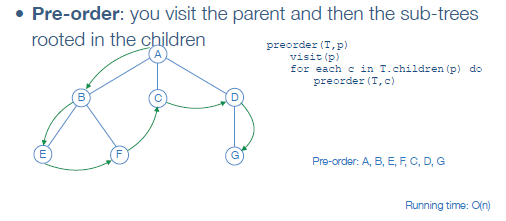
\includegraphics[width=0.75\linewidth]{immagini/tree1.png}
\end{figure}


\subsection{Post-order Traversal}
In \textbf{post-order traversal}, the children are visited before the parent.
\begin{verbatim}
postorder(T, p):
    for each c in T.children(p):
        postorder(T, c)
    visit(p)
\end{verbatim}
\begin{figure}[h!]
    \centering
    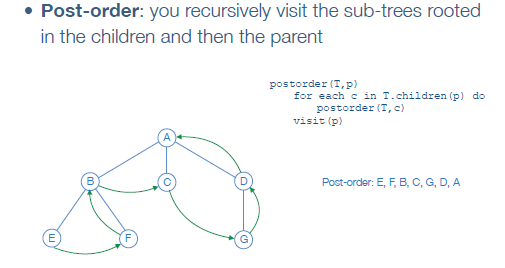
\includegraphics[width=0.75\linewidth]{immagini/tree2.png}
\end{figure}
\newpage
\subsection{Breadth-First Traversal (BFT)}
In \textbf{Breadth-First Traversal}, nodes are visited by depth level. This returns a tree. Not always it starts from left, it chooses a random child.
\begin{verbatim}
BFT(T):
    Q.enqueue(T.root())
    while not Q.is_empty():
        p = Q.dequeue()
        visit(p)
        for each c in T.children(p):
            Q.enqueue(c)
\end{verbatim}
\begin{figure}[h!]
    \centering
    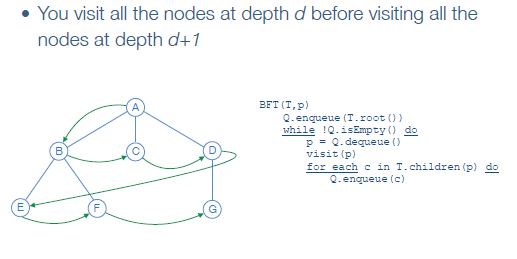
\includegraphics[width=0.75\linewidth]{immagini/tree3.png}
\end{figure}

\subsection{Exercise}
\begin{figure}[h!]
    \centering
    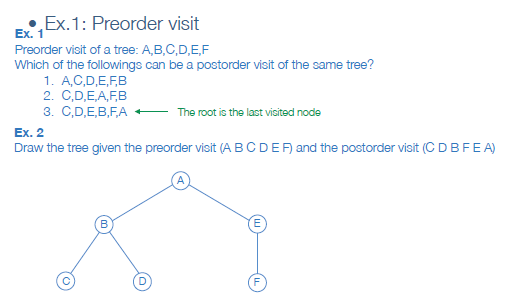
\includegraphics[width=1\linewidth]{immagini/tree4.png}
\end{figure}

\section{Binary Trees and Binary Search Trees (BST)}
A \textbf{binary tree} has each node with at most two children (left and right), the left child comes before the right child in the order of children of a node.
A binary tree is called \textbf{proper(or full)} if every node has zero or two children.
\begin{figure}[h!]
    \centering
    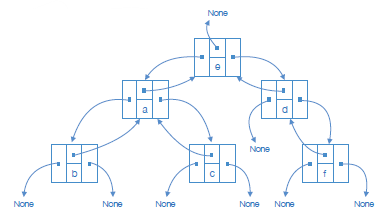
\includegraphics[width=0.75\linewidth]{immagini/tree5.png}
\end{figure}
A \textbf{Binary Search Tree (BST)} is an ordered binary tree where:
\begin{itemize}
    \item For any node \( x \), nodes in the left subtree of \( x \) have keys \( \leq x \).
    \item Nodes in the right subtree have keys \( \geq x \).
\end{itemize}
In other words: is a rooted binary tree data structure whose internal nodes each store a key greater than all the keys in
the node’s left subtree and less than those in its right subtree.

\paragraph{Complete and Full Binary Trees} There are many types of binary trees, but we will focus on two: complete and full.
\begin{itemize}
    \item \textbf{Full binary tree}: Every node has either 0 or 2 children.
    \item \textbf{Complete binary tree}: Every node has either 0 or 2 children, except for the last level, which may have some missing nodes. These nodes must be filled from left to right. A complete binary tree is also a heap.
\end{itemize}


\subsection{Binary Tree Traversal: In-Order}
In-order traversal for BST visits nodes from left to right:
\begin{verbatim}
inorder(T, x):
    if x is not None:
        inorder(T, x.left)
        visit(x)
        inorder(T, x.right)
\end{verbatim}
\begin{figure}[h!]
    \centering
    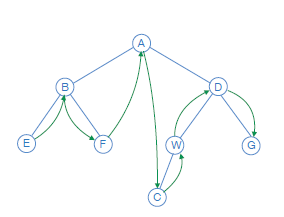
\includegraphics[width=0.6\linewidth]{immagini/tree6.png}
\end{figure}
\section{BST Operations}
Key operations in a BST include:
\begin{itemize}
    \item \textbf{Search}: Finding a node with a given key.
    \item \textbf{Minimum and Maximum}: Finding the smallest or largest element. By keeping going down to the left you will find the minimum, by going to the right you will find the maximum.
    \item \textbf{Successor and Predecessor}: Finding the next or previous node in sorted order.
\end{itemize}
\subsection{Binary Search Example: Tree-Search}
Searching for a key \( k \) in a BST starting from root node \( x \). Inputs: x is a given node where the search starts (usually the root) and k is the key to be searched in the tree. Outputs: a pointer to a node with key k or NIL if the key is not in the tree.

\begin{verbatim}
TREE-SEARCH(x, k):
    if x == NIL or k == x.key:
        return x
    if k < x.key:
        return TREE-SEARCH(x.left, k)
    else:
        return TREE-SEARCH(x.right, k)

ITERATIVE-TREE-SEARCH(x,k):
    while x!=NIL and k!=x.key() do
        if k<x.key
            x = x.left
        else
            x = x.right
    return x
\end{verbatim}

\begin{figure}[h!]
    \centering
    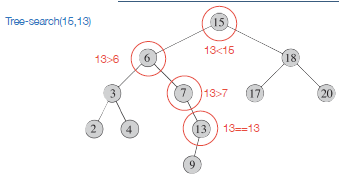
\includegraphics[width=0.75\linewidth]{immagini/tree7.png}
\end{figure}
The nodes encountered during the process form a path downward from the root, thus we visit a number of nodes which equals the height of the node k in the tree. Complexity: O(h) where h is the height
\newpage Exercise: Suppose we have numbers between 1 and 1000 in a binary search tree, and we want to search for the number 364. Which of the following sequences cannot be the sequence of nodes examined?
\begin{itemize}
    \item 1,252,401,398,330,344,397,364
    \item 924,220,911,244,898,258,362,364
    \item 925,202,911,240,912,245,364
\end{itemize}
There answer is the third option since 912 cannot belong to the left subtree of 911.

\subsection{Successor: Property}
Given a binary search tree \( T \) and \(x, y \) in \( T \) 
Given a binary search tree T and x,y in T, then \( y \) is a successor of \( x \) if \( y.key>x.key \) and there not exist a
 \( z \) in \( T \) such that \(  y.key> z.key >x.key\).  $\\$
 
\textbf{Property:} Consider a binary search tree T whose keys are distinct. If the right subtree of a node \(x\) in \(T\) is empty and \(x\) has a successor \(y\), then \(y\) is the lowest ancestor of \(x\) whose left child is also an ancestor-orself
of \(x\).
Note: in this case we consider a node to be an ancestor of itself.
The running time is O(h) since we either follow a simple path downwards or a simple path upwards.
\begin{figure}[h!]
    \centering
    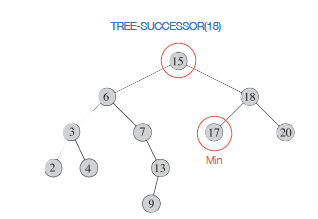
\includegraphics[width=0.75\linewidth]{immagini/tree8.png}
\end{figure}

    



\chapter{Markov Chains}
    
\chapter{Hash Tables}

\section{Direct-Address Table}
Direct addressing is a simple and efficient method when the universe \( U \) of possible keys is relatively small. A direct-address table \( T \) is an array where:
\[
T[i] = \text{value associated with key } i
\]
Given \( U = \{0, 1, \dots, m-1\} \), \( T \) is of size \( m \).

\subsection{Operations}
\begin{figure}[H]
    \centering
    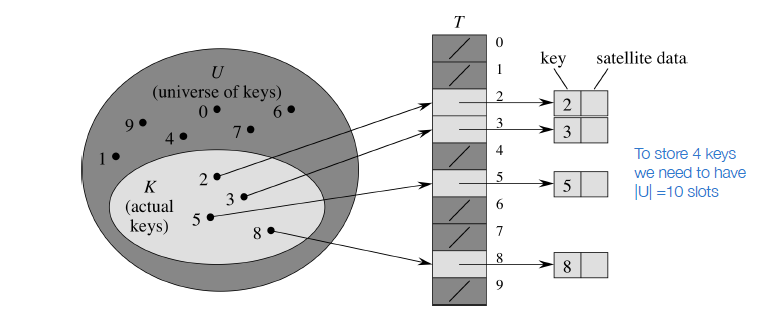
\includegraphics[width=0.75\linewidth]{direct-adress table.png}
    \label{fig:enter-label}
\end{figure}

\begin{itemize}
    \item \texttt{Direct-Table-Search(T, k):} Returns \( T[k] \), \( O(1) \).
    \item \texttt{Direct-Table-Insert(T, x):} Returns \( T[x.key] = x \), \( O(1) \).
    \item \texttt{Direct-Table-Delete(T, x):} Returns \( T[x.key] = NIL \), \( O(1) \).
\end{itemize}



While the first is a time-efficient approach, the 2nd and 3rd approaches becomes space-inefficient if \( |U| \gg |K| \), where \( K \) is the actual set of keys.

\section{Hash Tables}
Hash tables address the inefficiency of direct addressing by using a hash function \( h: U \to \{0, 1, \dots, m-1\} \), which maps keys to slots of a fixed-size table \( T[0,1,...,m-1] \). $\\$



\title{Hash Tables Overview}

\begin{itemize}
    \item Hash tables use a table size proportional to \( |K| \), losing the direct address ability.
    \item Direct-addressing maps \( k \to T[k] \), but wastes space if \( U \) (key space) is large.
    \item A \textbf{hash function} \( h \) maps keys to table slots:
    \[
    h : U \to \{ 0, 1, \dots, m-1 \}
    \]
    \item Keys are placed in \( T[h(k)] \) instead of \( T[k] \), optimizing storage.
\end{itemize}




\subsection{Hash Function}
A hash function should:
\begin{itemize}
    \item Be simple and fast to compute.
    \item Avoid collisions.
    \item Distribute keys evenly among cells.
\end{itemize}
Example: Let \( h(k) = k \mod 6 \), \( T[0..5] \):
\begin{itemize}
    \item Insert 7: \( 7 \mod 6 = 1 \)
    \item Insert 18: \( 18 \mod 6 = 0 \)
    \item Insert 41: \( 41 \mod 6 = 5 \)
    \item Insert 34: \( 34 \mod 6 = 4 \)
    \item Insert 10: \( 10 \mod 6 = 4 \) (collision with \( 34 \)).
\end{itemize}

\begin{figure}[H]
    \centering
    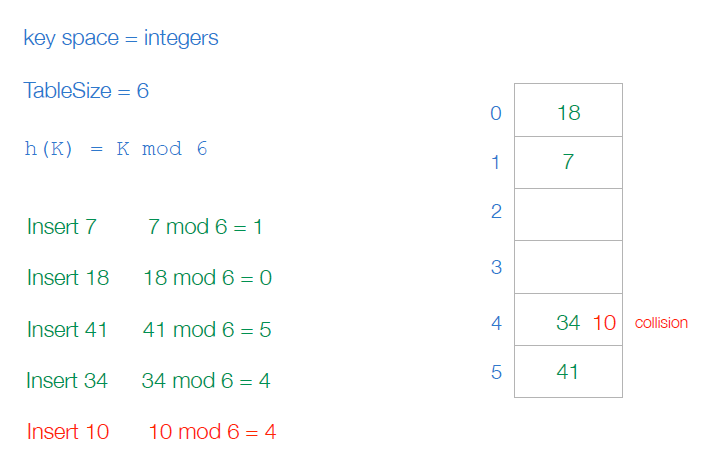
\includegraphics[width=0.75\linewidth]{hash function exam.png}
    \label{fig:enter-label}
\end{figure}


\section{Collision Resolution Strategies}

\subsection{Separate Chaining}
Collisions are resolved by maintaining a linked list at each slot.
\begin{itemize}
    \item \texttt{Insert:} \( O(1) \) if the element is unique, otherwise \( O(1 + \text{SEARCH}) \).
    \item \texttt{Search:} Proportional to the list length at the slot.
    \item \texttt{Delete:} \( O(1 + \text{SEARCH}) \).
\end{itemize}
Performance depends on the \textbf{load factor} \( \alpha = \frac{n}{m} \), where \( n \) is the number of elements and \( m \) is the size of the table. $\\$
The load factor is the average number of elements stored in a hash table where \(\alpha \in[0,1]\). Therefore the worst case is $\Theta (n)$.

\begin{figure}[H]
    \centering
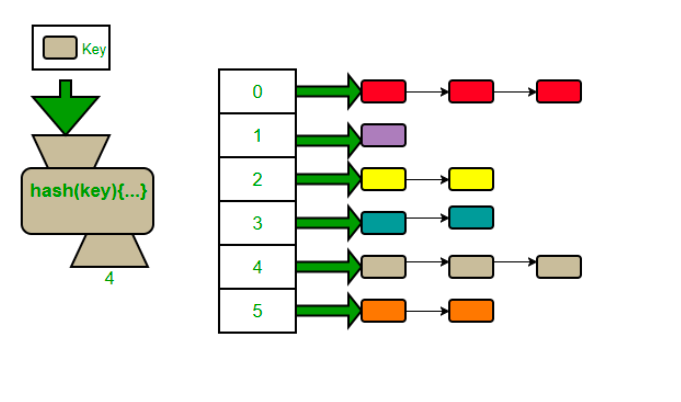
\includegraphics[width=0.75\linewidth]{separe chaining.png}
\end{figure}



\section{Simple Uniform Hashing}

\begin{itemize}
    \item For \( j = 0, 1, \dots, m-1 \), let \( T[j] \) denote the list corresponding to slot \( j \) with length \( n_j \), such that:
    \[
    n = n_0 + n_1 + \dots + n_{m-1}.
    \]
    \item The expected value of \( n_j \) is:
    \[
    \mathbb{E}[n_j] = \alpha = \frac{n}{m},
    \]
    where \( \alpha \) is the load factor.
    \item The average running time for a successful search in a hash table using chaining and assuming simple uniform hashing is:
    \[
    \Theta(1 + \alpha).
    \]
    \item If \( m \) is proportional to \( n \), then \( n = O(m) \) and:
    \[
    \alpha = \frac{n}{m} = \frac{O(m)}{m} = O(1).
    \]
\end{itemize}



\subsection*{Division Method}
The hash function is defined as:
\[
h(k) = k \mod m
\]
where \( k \) is the key, and \( m \) is the table size. 
\begin{itemize}
    \item Choose \( m \) as a prime number not close to a power of 2.
    \item Example: For \( n = 2000 \) keys and 3 collisions per list, estimate \( m \approx 666 \). A good choice is \( m = 701 \).
\end{itemize}

\subsection{Alternative Methods}
\begin{itemize}
    \item \textbf{Multiplication Method}:
    \[
    h(k) = \lfloor m \cdot (kA \mod 1) \rfloor
    \]
    where \( A \approx 0.61803 \) (Knuth's suggestion).
   \item \textbf{Squaring Method}:
    \begin{itemize}
        \item Square the key and extract middle bits.
        \item Often use \( m = 2^p \) for simpler computation.
    \end{itemize}

\end{itemize}







\subsection{Open Addressing}
Instead of linked lists (which requires the implementation of a second data structure), all data is stored directly in the table (we need a bigger table and the load factor should be below 0.5). When a collision occurs, alternative cells are probed until an empty slot is found.
Strategies include:
\begin{enumerate}
    \item \textbf{Linear Probing:} \( h_i(k) = (h(k) + i) \mod m \).
    \item \textbf{Quadratic Probing:} \( h_i(k) = (h(k) + i^2) \mod m \).
    \item \textbf{Double Hashing:} \( h_i(k) = (h(k) + i \cdot g(k)) \mod m \), where \( g \) is a second hash function.
\end{enumerate}

\subsubsection{Linear Probing Example}

\textbf{Probe Sequence:}  
When resolving collisions using linear probing, the probe sequence is defined as follows:

\begin{itemize}
    \item \( 0^\text{th} \) probe: \( h(k) = k \mod \text{TableSize} \),
    \item \( 1^\text{st} \) probe: \( (h(k) + 1) \mod \text{TableSize} \),
    \item \( 2^\text{nd} \) probe: \( (h(k) + 2) \mod \text{TableSize} \),
    \item \(\dots\),
    \item \( i^\text{th} \) probe: \( (h(k) + i) \mod \text{TableSize} \).
\end{itemize}
\textbf{Key Properties:}
\begin{itemize}
    \item A function of \( i \) is added to the original hash value to resolve collisions.
    \item Any key that hashes into an existing cluster:
    \begin{enumerate}
        \item Will require multiple attempts to resolve the collision.
        \item Will contribute to the cluster, increasing its size.
    \end{enumerate}
\end{itemize}


\begin{figure}[H]
    \centering
    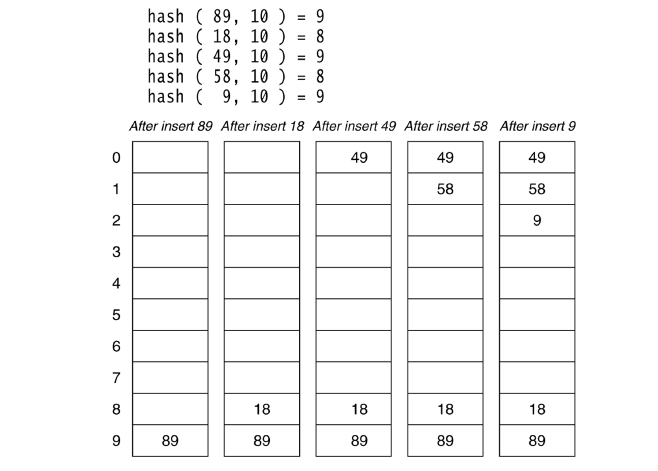
\includegraphics[width=0.75\linewidth]{linear probing.png}
\end{figure}




\subsection{Open Addressing: Search and Insertion}  

In open addressing, the search process uses the same probe sequence as insertion. For example, searching for 58 takes 4 probes, while searching for 19 takes 5.  

The average number of cells examined during insertion with linear probing is:  
\[
\frac{1 + \frac{1}{(1 - \alpha)^2}}{2}
\]  
The cost of successfully searching for an element equals the cost of its insertion.  

When the table is half full (\( \alpha = 0.5 \)), the average insertion cost is 2.5, and this remains true for future searches.  

For unsuccessful searches, the average cost is:  
\[
\frac{1 + \frac{1}{(1 - \alpha)^2}}{2}
\]  
For successful searches:  
\[
\frac{1 + \frac{1}{1 - \alpha}}{2}
\]  
At \( \alpha = 0.5 \), insertion typically examines 2.5 cells.  

Primary clustering worsens as the table fills, but when half empty, the effect is minimal.  

\subsection{Linear Probing Example:}
\begin{figure}[H]
    \centering
    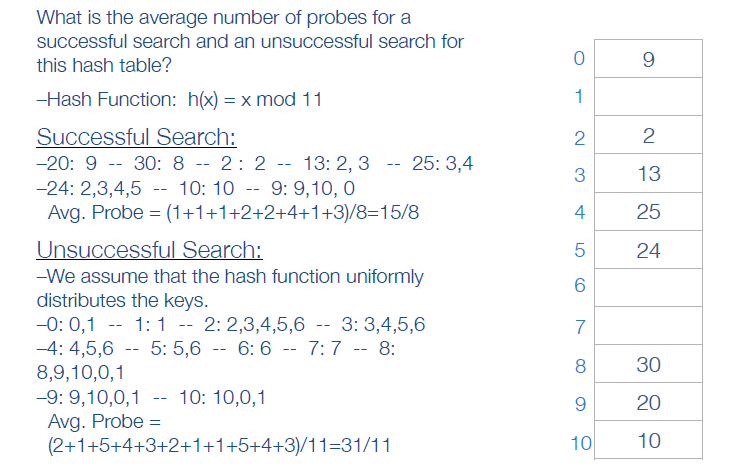
\includegraphics[width=0.75\linewidth]{LP example.png}
\end{figure}

\subsubsection{Primary Clustering}
It works pretty well for an empty table and gets worse as the table fills up.
If a bunch of elements hash to the same spot, they clash with each other. But, worse, if a bunch of elements hash to the same area of the table, they keep clashing! (Even though the hash function isn’t producing lots of collisions!)$\\$
This phenomenon is called primary clustering and Linear probing suffers from \textbf{primary clustering}, where elements form clusters that grow, increasing the likelihood of future collisions.

\begin{figure}[H]
    \centering
    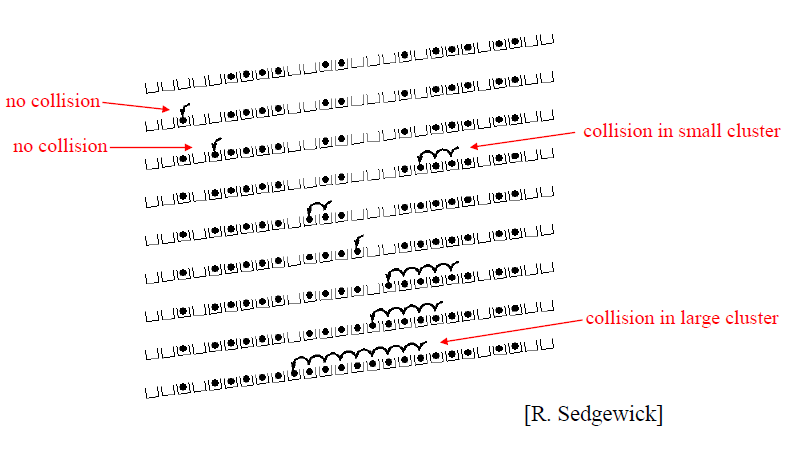
\includegraphics[width=0.75\linewidth]{primary clustering.png}
    \caption{Enter Caption}
    \label{fig:enter-label}
\end{figure}

\subsubsection{Quadratic Probing}
\textbf{Reduces Primary Clustering:} Keys that hash to nearby slots do not follow the same probe sequence.

Reduces clustering but may encounter \textbf{secondary clustering} where keys hashing to the same slot follow identical probe sequences. \( h_i(k) = (h(k) + i^2) \mod m \).

There are cases in which, due to probing, there is no available spot. If there are numbers in the same place those will cause infinite collisions. For example
\begin{align}
47 \hspace{1mm} \text{mod} \hspace{1mm} 7 =  5 \rightarrow & 5+(i^2) \\
                                               \rightarrow & 5+(i+1)^2 \\
                                               \rightarrow & 5+(i+2)^2 ...    
\end{align}
but also
\begin{align}
75 \hspace{1mm} \text{mod} \hspace{1mm} 7 =  5 \rightarrow & 5+(i^2) \\
                                               \rightarrow & 5+(i+1)^2 \\
                                               \rightarrow & 5+(i+2)^2 ...    
\end{align}
\begin{figure}[h!]
    \centering
    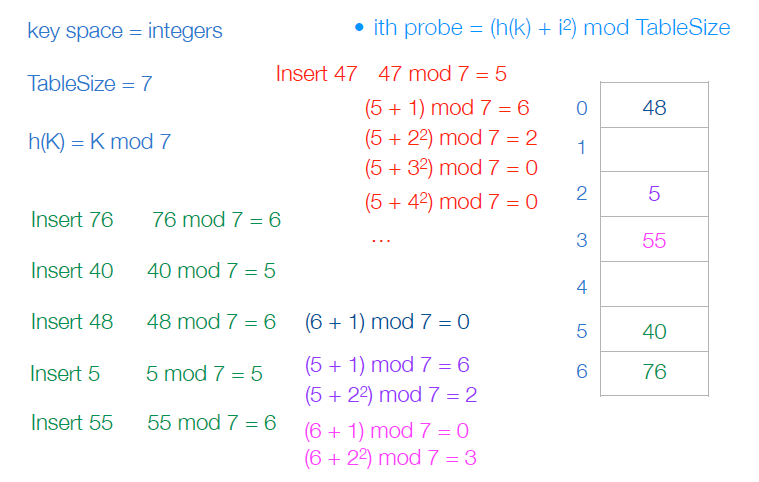
\includegraphics[width=0.75\linewidth]{quadratic probing example.png}
    \label{fig:enter-label}
\end{figure}

\subsubsection{Double Hashing Example}
Hash function \( h(k) = k \mod 7 \), \( g(k) = 5 - (k \mod 5) \):
Insert 76, 93, 40, 47, 10, 55. \newline
\textbf{Table Size:}  
 Optimal load factor \( \alpha = \frac{1}{2} \) (table twice as large as expected elements).  \newline
\textbf{Probe Calculation} Next probe:  
    \[
    (i+1)^2 - i^2 = 2i + 1
    \]
For \( \alpha < \frac{1}{2} \), an empty slot is always found. If \( \alpha > \frac{1}{2} \), a slot may not exist.  

\begin{figure}[h!]
    \centering
    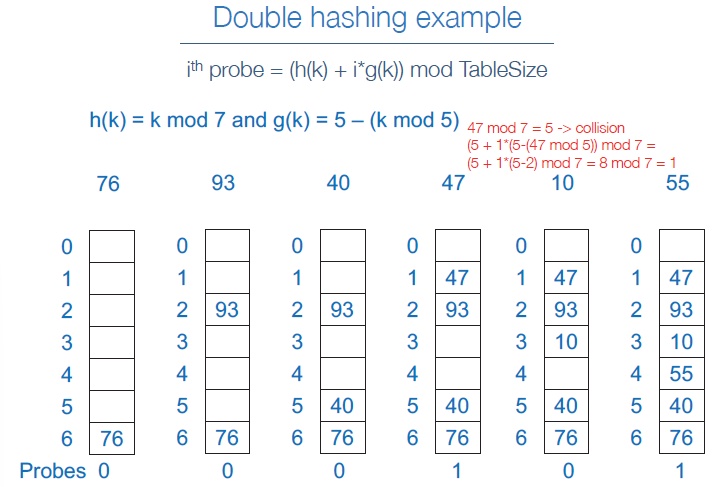
\includegraphics[width=0.75\linewidth]{immagini/doublehahing.png}
\end{figure}
\section{Rehashing}
When the table is too full (\( \alpha > 0.5 \)), rehashing is required:
\begin{itemize}
    \item Create a new table, typically twice as large.
    \item Recompute hash values for all non-deleted keys.
\end{itemize}
Rehashing costs \( O(n) \) but occurs infrequently.

\section{Python Hash Tables}
Python dictionaries are implemented as hash tables using \textbf{open addressing:}  with random probing. Collisions are handled by comparing both the hash and the key. If the hash and key match, the entry is skipped, otherwise probing continues until an empty slot is found. 
$\\$

When a new dictionary is created, it starts with 8 slots. The table resizes when it becomes two-thirds full to maintain efficiency. Each slot can store one entry, and if the slot is occupied, Python checks for a match using the == operator (not is). If no match is found, random probing selects the next slot in a pseudo-random order, continuing until the entry is placed. 
$\\$

This design ensures efficient insertion, lookup, and handling of collisions, keeping Python dictionaries fast and reliable.

\chapter{Martingale}
    \chapter{Heaps and Heapsort}

\section{Introduction to Heaps}
\begin{figure}[h!]
    \centering
    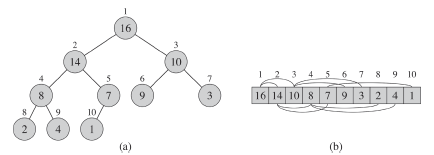
\includegraphics[width=0.75\linewidth]{immagini/heap1.png}
\end{figure}
Heaps are a foundational data structure in computer science used for efficient sorting and priority management. They offer:
\begin{itemize}
    \item Sorting algorithm with \( O(n \log n) \) complexity.
    \item An in-place sorting mechanism.
    \item A design that uses a specific data structure to manage information during execution.
    \item Applications in sorting (\textit{Heapsort}) and other efficient structures like priority queues.
\end{itemize}

\section{The Heap Data Structure}
A \textbf{heap} is an array-based data structure often represented as a nearly complete binary tree:
\begin{itemize}
    \item The tree is filled level by level, with the last level filled from left to right. The first element will always be the root.
    \item An array \( A \) representing a heap has attributes:
    \begin{itemize}
        \item \texttt{length[A]}: Total size of the array.
        \item \texttt{heap-size[A]}: Number of elements in the heap, with \( \texttt{heap-size[A]} \leq \texttt{length[A]} \).
    \end{itemize}
\end{itemize}
\begin{figure}[H]
    \centering
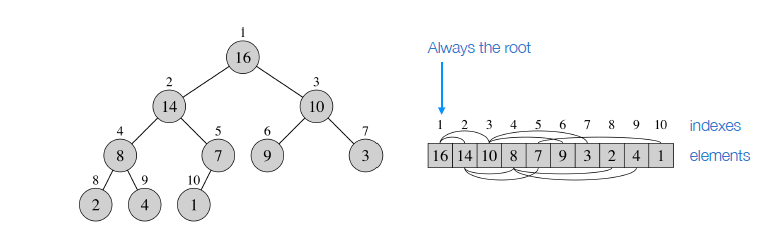
\includegraphics[width=0.8\linewidth]{Heap structure.png}
    \caption{}
    \label{fig:enter-label}
\end{figure}


\subsection{Heap Properties}
\begin{itemize}
    \item The root is stored at \( A[1] \).
    \item For an element at index \( i \):
    \begin{itemize}
        \item Parent: \( A[\lfloor i/2 \rfloor] \).
        \item Left child: \( A[2i] \).
        \item Right child: \( A[2i+1] \).
    \end{itemize}
    \item \textbf{Max-heap property:} \( A[\text{parent}(i)] \geq A[i] \).
    \item \textbf{Min-heap property:} \( A[\text{parent}(i)] \leq A[i] \).
\end{itemize}
\subsection{exercise}
\begin{figure}[h!]
    \centering
    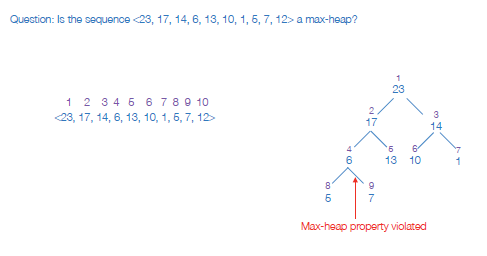
\includegraphics[width=1\linewidth]{immagini/heap2.png}
\end{figure}

\begin{figure}[H]
    \centering
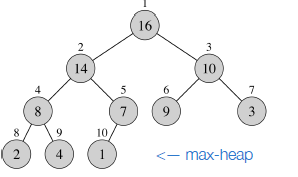
\includegraphics[width=0.5\linewidth]{heap prop.png}
    \label{fig:enter-label}
\end{figure}


\section{Max-Heapify}
The \textbf{Max-Heapify} operation ensures the max-heap property by adjusting the heap from a specific index downward.

\subsection{Algorithm: Max-Heapify}
\begin{verbatim}
MAX-HEAPIFY(A, i)
l = left(i)
r = right(i)
if l <= heap-size[A] and A[l] > A[i] then
    largest = l
else
    largest = i
if r <= heap-size[A] and A[r] > A[largest] then
    largest = r
if largest != i then
    exchange A[i] with A[largest]
    MAX-HEAPIFY(A, largest)
\end{verbatim}

\textbf{Complexity:} \( O(\log n) \), proportional to the height of the tree.
\begin{figure}[h!]
    \centering
    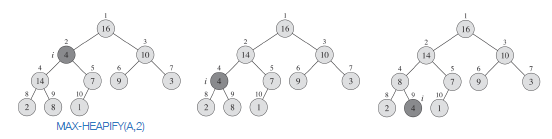
\includegraphics[width=1\linewidth]{immagini/heap3.png}
\end{figure}
\section{Building a Max-Heap}
\textbf{BUILD-MAX-HEAP} constructs a max-heap from an unordered array.

\subsection{Algorithm: Build-Max-Heap}
\begin{verbatim}
BUILD-MAX-HEAP(A)
heap-size[A] = length[A]
for i = floor(length[A]/2) downto 1 do
    MAX-HEAPIFY(A, i)
\end{verbatim}
\textbf{Complexity:} \( O(n) \). This is more efficient than the naive \( O(n \log n) \) bound because most heap levels have fewer nodes. \newline
\textbf{How does it work?} The algorithm starts checking from the element $\lfloor len(A)/2 \rfloor$ and then works its way back up. In each step, it fixes everything before moving on. Note that the system always looks down and not up, using \textbf{MAX-HEAPIFY(A,1)} we always consider the first element that looks at the entire graph.
\subsection{Exercise}
    \begin{figure}[h!]
        \centering
        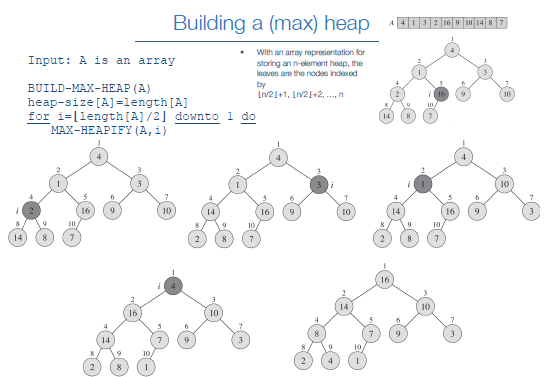
\includegraphics[width=1\linewidth]{immagini/heap4.png}
    \end{figure}
The loop could not go from 1 to floor(length[A]/2) because it could not guarantee the maxheap property. E.g. A [2,1,1,3] then MAX-HEAPIFY won’t exchange 2 with it’s children (1’s). However, when MAX-HEAPIFY is called on the left child, 1, it will swap 1 with 3. This violates the max-heap property because now 2 is the parent of 3. An upper bound of the running time is O(n log n) because MAX-HEAPIFY costs O(log n) and we call it O(n) times. It is possible to derive a tighter upper bound by observing that the time required by MAXHEAPIFY varies with the height of the node and most heights are small. It can be proved that BUILD-MAX-HEAP run in O(n).
    
\section{Heapsort}
\textbf{Heapsort} is a sorting algorithm that uses a heap to organize data efficiently.

\subsection{Algorithm: Heapsort}
\begin{verbatim}
HEAPSORT(A)
BUILD-MAX-HEAP(A) #O(n)
for i = len(A) downto 2 do #O(n-1)
    exchange A[1] with A[i] #O(1)
    A.heap-size = A.heap-size - 1 #O(1)
    MAX-HEAPIFY(A, 1) #O(logn)
\end{verbatim}
\textbf{Complexity:} \( O(n) + O((n-1)(\log n)) = O(n \log n) \).

\subsection{Exercise 1}
    \begin{figure}[h!]
        \centering
        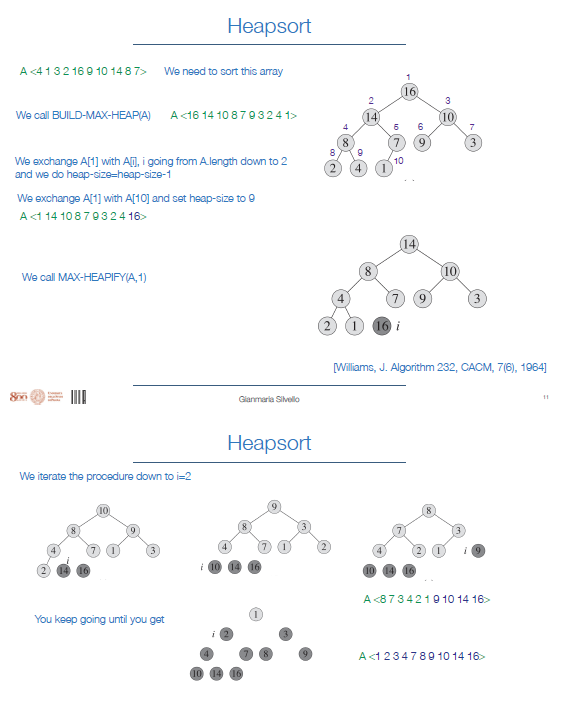
\includegraphics[width=1\linewidth]{immagini/heap5.png}
    \end{figure}
\newpage
\subsection{Exercise 2}
    \begin{figure}[h!]
        \centering
        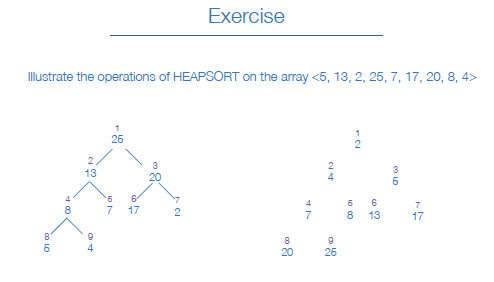
\includegraphics[width=0.8\linewidth]{immagini/heap6.png}
    \end{figure}

\section{Priority Queues}
Priority queues are abstract data structures for managing elements with associated priorities.

\subsection{Operations}
\begin{itemize}
    \item \texttt{INSERT(S, x)}: Add element \( x \) to \( S \).
    \item \texttt{MAXIMUM(S)}: Return the element with the maximum key.
    \item \texttt{EXTRACT-MAX(S)}: Remove and return the element with the maximum key.
    \item \texttt{INCREASE-KEY(S, x, k)}: Increase the key of \( x \) to \( k \) (\( k \geq \) current key).
\end{itemize}

\subsection{Complexity}
If implemented with a heap:
\begin{itemize}
    \item \texttt{INSERT(S, x)}: \( O(\log n) \).
    \item \texttt{MAXIMUM(S)}: \( O(1) \).
    \item \texttt{EXTRACT-MAX(S)}: \( O(\log n) \).
\end{itemize}

%\chapter{Formulary}
%    \section*{1. Bernoulli Distribution}
\textbf{Distribution:} \( X \sim \text{Bernoulli}(p) \), where \( p \) is the probability of success in a single trial.\\
\textbf{Probability Mass Function (PMF):}
\[
P(X = x) = 
\begin{cases} 
p & \text{if } x = 1 \\ 
1 - p & \text{if } x = 0 
\end{cases}
\]
\textbf{Cumulative Distribution Function (CDF):}
\[
F(x) = 
\begin{cases} 
0 & \text{if } x < 0 \\ 
1 - p & \text{if } 0 \le x < 1 \\ 
1 & \text{if } x \ge 1 
\end{cases}
\]
\textbf{Expectation:} \( \mathbb{E}[X] = p \)\\
\textbf{Variance:} \( \operatorname{Var}(X) = p(1 - p) \)

\section*{2. Binomial Distribution}
\textbf{Distribution:} \( X \sim \text{Binomial}(n, p) \), with \( n \) trials and probability of success \( p \) per trial.\\
\textbf{Probability Mass Function (PMF):}
\[
P(X = k) = \binom{n}{k} p^k (1 - p)^{n - k}, \quad k = 0, 1, \ldots, n
\]
\textbf{Cumulative Distribution Function (CDF):}
\[
F(k) = \sum_{j=0}^{k} \binom{n}{j} p^j (1 - p)^{n - j}
\]
\textbf{Expectation:} \( \mathbb{E}[X] = np \)\\
\textbf{Variance:} \( \operatorname{Var}(X) = np(1 - p) \)

\section*{3. Geometric Distribution}
\textbf{Distribution:} \( X \sim \text{Geom}(p) \), where \( p \) is the probability of success.\\
\textbf{Probability Mass Function (PMF):}
\[
P(X = k) = (1 - p)^{k - 1} p, \quad k = 1, 2, \ldots
\]
\textbf{Cumulative Distribution Function (CDF):}
\[
F(k) = 1 - (1 - p)^k
\]
\textbf{Expectation:} \( \mathbb{E}[X] = \frac{1}{p} \)\\
\textbf{Variance:} \( \operatorname{Var}(X) = \frac{1 - p}{p^2} \)

\section*{4. Poisson Distribution}
\textbf{Distribution:} \( X \sim \text{Poisson}(\lambda) \), where \( \lambda \) is the average rate of occurrence.\\
\textbf{Probability Mass Function (PMF):}
\[
P(X = k) = \frac{\lambda^k e^{-\lambda}}{k!}, \quad k = 0, 1, 2, \ldots
\]
\textbf{Cumulative Distribution Function (CDF):}
\[
F(k) = e^{-\lambda} \sum_{j=0}^{k} \frac{\lambda^j}{j!}
\]
\textbf{Expectation:} \( \mathbb{E}[X] = \lambda \)\\
\textbf{Variance:} \( \operatorname{Var}(X) = \lambda \)

\section*{5. Normal Distribution}
\textbf{Distribution:} \( X \sim \text{Normal}(\mu, \sigma^2) \), with mean \( \mu \) and variance \( \sigma^2 \).\\
\textbf{Probability Density Function (PDF):}
\[
f(x) = \frac{1}{\sqrt{2 \pi \sigma^2}} e^{-\frac{(x - \mu)^2}{2 \sigma^2}}
\]
\textbf{Cumulative Distribution Function (CDF):}
\[
F(x) = \frac{1}{2} \left[ 1 + \operatorname{erf}\left( \frac{x - \mu}{\sigma \sqrt{2}} \right) \right]
\]
\textbf{Expectation:} \( \mathbb{E}[X] = \mu \)\\
\textbf{Variance:} \( \operatorname{Var}(X) = \sigma^2 \)

\section*{6. Exponential Distribution}
\textbf{Distribution:} \( X \sim \text{Exp}(\lambda) \), where \( \lambda \) is the rate parameter.\\
\textbf{Probability Density Function (PDF):}
\[
f(x) = \lambda e^{-\lambda x}, \quad x \geq 0
\]
\textbf{Cumulative Distribution Function (CDF):}
\[
F(x) = 1 - e^{-\lambda x}, \quad x \geq 0
\]
\textbf{Expectation:} \( \mathbb{E}[X] = \frac{1}{\lambda} \)\\
\textbf{Variance:} \( \operatorname{Var}(X) = \frac{1}{\lambda^2} \)

\section*{7. Continuous Uniform Distribution}
\textbf{Distribution:} \( X \sim \text{Uniform}(a, b) \), where \( a \) and \( b \) are the interval endpoints.\\
\textbf{Probability Density Function (PDF):}
\[
f(x) = \frac{1}{b - a}, \quad x \in [a, b]
\]
\textbf{Cumulative Distribution Function (CDF):}
\[
F(x) = 
\begin{cases} 
0 & \text{if } x < a \\ 
\frac{x - a}{b - a} & \text{if } a \le x \le b \\ 
1 & \text{if } x > b 
\end{cases}
\]
\textbf{Expectation:} \( \mathbb{E}[X] = \frac{a + b}{2} \)\\
\textbf{Variance:} \( \operatorname{Var}(X) = \frac{(b - a)^2}{12} \)
\end{document}